\chapter{Esperimenti}

\section{Cluster ChemGrid}

Tutti gli esperimenti sono stati eseguiti sul cluster ChemGrid. Il cluster \`{e} composto da 11 nodi a 32 bit con 2 processori Intel(R) Pentium(R) 4 CPU 3.06GHz. Tutti i nodi hanno 1GB di memoria tranne 4 nodi (8, 9 10, 11) che hanno 4GB. 3 nodi (3, 6, 11) sono offline e dunque non utilizzabili per sottomettere job. Dunque i nodi utilizzabili sono 8 per un totale di 16 CPU.

Da ricordare che ci serve un quadrato perfetto per eseguire l'algoritmo di Cannon: 4, 9 e 16 sono i possibili candidati. 9 non \`{e} possibile utilizzarlo perch\`{e} non si hanno a disposizione sufficienti host.
Il 4 potrebbe essere derivato da 4 host con una sola CPU oppure da 2 host con 2 CPU. Infine 16 \`{e} ottenibile solo con 8 host a 2 CPU l'uno.
Tutti gli esperimenti verranno eseguiti con questa ultima configurazione: 8 host e 2 CPU per nodo, per un totale di 16 CPU.

\section{Data file}

Il file di input utilizzato per gli esperimenti ha le seguenti dimensioni:

\begin{lstlisting}
4 4 4 2
8 8 8 2
16 16 16 2
32 32 32 2
64 64 64 2
128 128 128 2
192 192 192 2
256 256 256 2
384 384 384 2
512 512 512 2
768 768 768 2
1024 1024 1024 2
1536 1536 1536 2
2048 2048 2048 2
3072 3072 3072 2
4096 4096 4096 2
\end{lstlisting}

Non ha senso andare oltre 4096 perch\`{e} la computazione inizia ad essere impegnativa impiegando tutte le risorse del cluster e, come si vedr\`{a} in seguito le prestazioni iniziano ad essere stabili dal 1024.

Si consideri che una matrice quadrata con n = 4096 ha 134217728 elementi. Ogni elemento \`{e} un double che occupa 8 bytes, dunque una matrice occupa circa 131Mb.

Tutti i test sono stati fatti utilizzando 2 iterazioni.

Per ogni esperimento verranno mostrati due grafici: uno dei tempi di esecuzione di colore blu e l'altro di colore rosso che rappresenta il throughput in Gflop/s. Il throughput \`{e} calcolato nel seguente modo:

\vspace{5mm}
$gflop/s = \frac{2 * n^3}{time} * 1.0e-9$
\vspace{5mm}

Dove \textit{time} \`{e} la media dei tempi tra le due iterazioni.

\subsection{Seriale}

La versione seriale \`{e} stata eseguita su un nodo (cg11) che ha 4GB di memoria per permettere alle dimensioni pi\`{u} grandi si essere moltiplicate senza problemi. Di seguito i suoi risultati:

\begin{lstlisting}
   n|        time|    Gflops/s
------------------------------
   4|      0.0000|  1.2800e-01
   8|      0.0000|  4.0960e-01
  16|      0.0000|  7.6205e-01
  32|      0.0001|  8.5250e-01
  64|      0.0006|  8.6170e-01
 128|      0.0045|  9.4038e-01
 192|      0.0163|  8.7050e-01
 256|      0.0409|  8.1963e-01
 384|      0.1301|  8.7073e-01
 512|      0.3523|  7.6190e-01
 768|      1.2080|  7.4996e-01
1024|      3.1203|  6.8823e-01
1536|     11.0251|  6.5739e-01
2048|     27.9096|  6.1555e-01
3072|     89.7327|  6.4616e-01
4096|    222.7798|  6.1693e-01
\end{lstlisting}

Le rappresentazioni grafiche dei dati sono nelle figure \ref{fig:x.mm_serial_1} e \ref{fig:x.mm_serial_2}.

\begin{figure}[htbp]
    \begin{center}
        \includegraphics[width=10cm]{immagini/{x.mm_serial_1}.png}
    \end{center}
    \caption{MM MPI seriale: tempo di esecuzione}
    \label{fig:x.mm_serial_1}
\end{figure}

\begin{figure}[htbp]
    \begin{center}
        \includegraphics[width=10cm]{immagini/{x.mm_serial_2}.png}
    \end{center}
    \caption{MM MPI seriale: Gflop/s}
    \label{fig:x.mm_serial_2}
\end{figure}

Si nota subito che l'andamento del tempo \`{e} esponenziale al crescere delle dimensioni delle matrici mentre il throughput si inizia a stabilizzare dalla matrice a 1024.
Per le matrici con dimensioni che vanno da 32 a 384 si hanno dei throughput migliori.

\subsection{Versione MPI bloccante}

Qui di seguito i risultati della version MPI \textbf{bloccante} senza alcuna ottimizzazione. Si ricorda che questa versione fa uso della primitivat MPI \textit{MPI\_Sendrecv\_replace()} e che utilizza un solo buffer sia per l'invio che per la ricezione.

\begin{lstlisting}
   n|        time|    Gflops/s
------------------------------
   4|      0.0247|  5.1870e-06
   8|      0.0138|  7.4089e-05
  16|      0.0083|  9.8622e-04
  32|      0.0057|  1.1505e-02
  64|      0.0054|  9.6908e-02
 128|      0.0073|  5.7146e-01
 192|      0.0131|  1.0801e+00
 256|      0.0233|  1.4377e+00
 384|      0.0514|  2.2017e+00
 512|      0.3167|  8.4772e-01
 768|      0.6362|  1.4241e+00
1024|      8.8529|  2.4257e-01
1536|     25.2136|  2.8745e-01
2048|    103.0118|  1.6678e-01
3072|    353.7942|  1.6389e-01
4096|    875.8602|  1.5692e-01
\end{lstlisting}

Le figure \ref{fig:x.mm_2d_cannon.o2295_1} e \ref{fig:x.mm_2d_cannon.o2295_2} sono le relative rappresentazioni grafiche per il tempo trascorso e la velocit\`{a} di trasmissione dei dati.

\begin{figure}[htbp]
    \begin{center}
        \includegraphics[width=10cm]{immagini/{x.mm_2d_cannon.o2295_1}.png}
    \end{center}
    \caption{MM MPI bloccante: tempo di esecuzione}
    \label{fig:x.mm_2d_cannon.o2295_1}
\end{figure}

\begin{figure}[htbp]
    \begin{center}
        \includegraphics[width=10cm]{immagini/{x.mm_2d_cannon.o2295_2}.png}
    \end{center}
    \caption{MM MPI bloccante: Gflop/s}
    \label{fig:x.mm_2d_cannon.o2295_2}
\end{figure}

Come nella versione seriale, si vede che i tempi di esecuzione crescono in maniera esponenziale e che dalla matrice 1024 il throughput si stabilizza.

\paragraph{Speedup ed efficienza}

Prima di calcolare speedup ed efficienza, si ricorda come vengono calcolati. Lo speedup \`{e} cos\`{i} definito:

\vspace{5mm}
$S(p) = \frac{T(1)}{T(p)}$
\vspace{5mm}

e misura la riduzione del tempo di esecuzione rispetto all'algoritmo seriale. L'efficienza invece \`{e} definita come:

\vspace{5mm}
$E(p) = \frac{S(p)}{p}$
\vspace{5mm}

e misura quanto l'algoritmo sfrutta il parallelismo del calcolatore. Ecco di seguito i risultati tra l'implementazione seriale e quella parallela bloccante.

\begin{lstlisting}
size| serial time|  paral time|     speedup|  efficiency
--------------------------------------------------------
   4|         0.0|      0.0247|      0.0000|      0.0000
   8|         0.0|      0.0138|      0.0000|      0.0000
  16|         0.0|      0.0083|      0.0000|      0.0000
  32|      0.0001|      0.0057|      0.0175|      0.0011
  64|      0.0006|      0.0054|      0.1111|      0.0069
 128|      0.0045|      0.0073|      0.6164|      0.0385
 192|      0.0163|      0.0131|      1.2443|      0.0778
 256|      0.0409|      0.0233|      1.7554|      0.1097
 384|      0.1301|      0.0514|      2.5311|      0.1582
 512|      0.3523|      0.3167|      1.1124|      0.0695
 768|       1.208|      0.6362|      1.8988|      0.1187
1024|      3.1203|      8.8529|      0.3525|      0.0220
1536|     11.0251|     25.2136|      0.4373|      0.0273
2048|     27.9096|    103.0118|      0.2709|      0.0169
3072|     89.7327|    353.7942|      0.2536|      0.0159
4096|    222.7798|    875.8602|      0.2544|      0.0159
\end{lstlisting}

La figura \ref{fig:speedup_serial_2d_cannon} mostra il grafico dello speedup tra le due implementazioni.

\begin{figure}[htbp]
    \begin{center}
        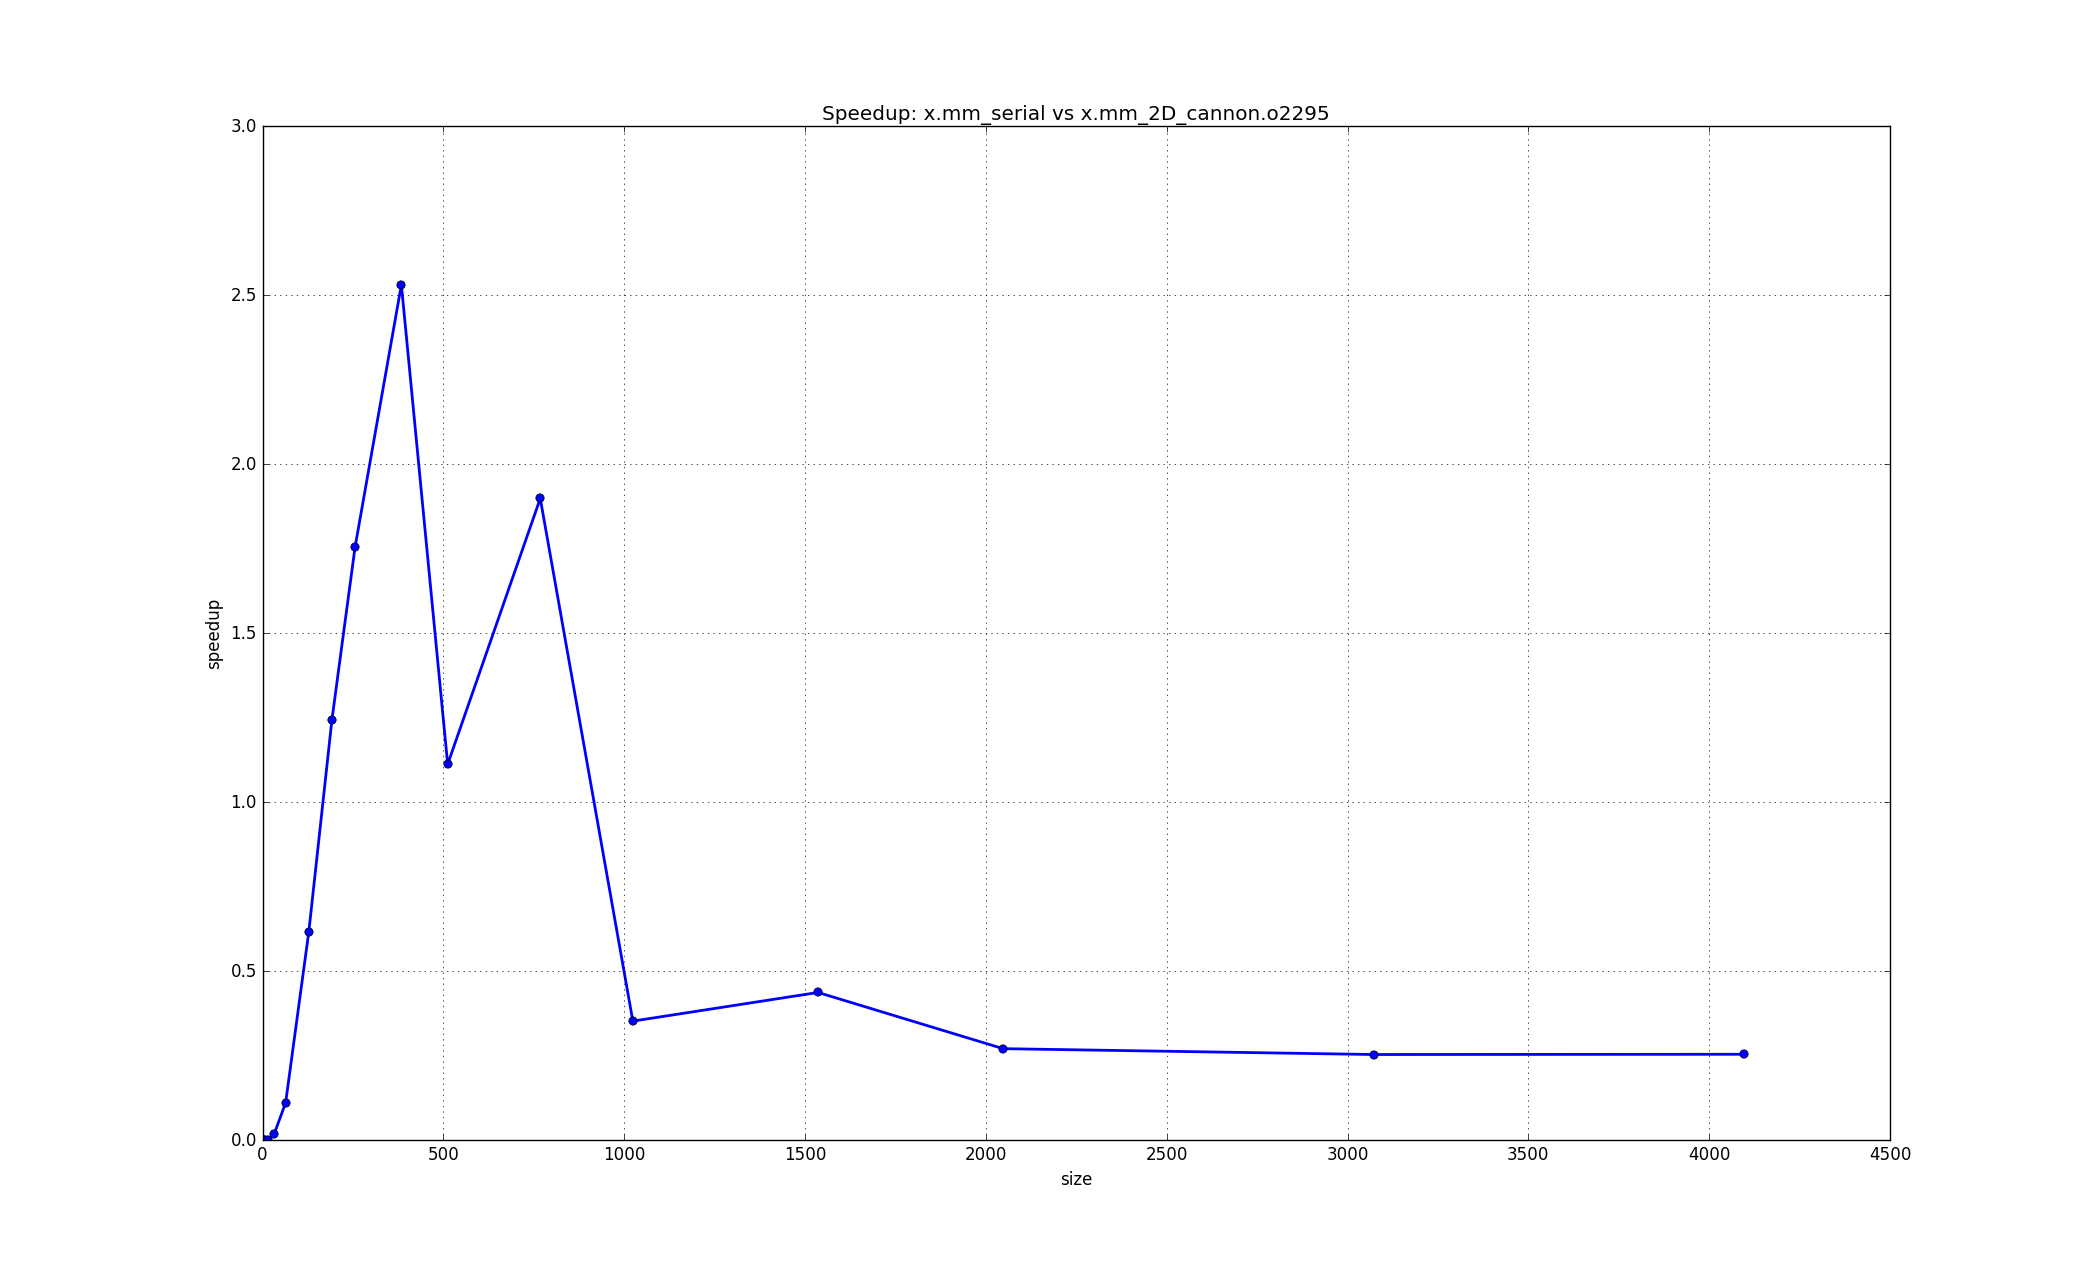
\includegraphics[width=15cm]{immagini/speedup_serial_2d_cannon.png}
    \end{center}
    \caption{Speedup seriale vs 2d cannon}
    \label{fig:speedup_serial_2d_cannon}
\end{figure}

Come si pu\`{o} vedere l'algoritmo ha uno speedup piuttosto basso tranne per le dimensioni che vanno da 192 a 768 che \`{e} maggiore di 1.
L'efficienza nel caso migliore non supera lo 0.15. Si pu\`{o} concludere che l'implementazione parallela bloccante non e` migliore rispetto alla corrispettiva parallela, tranne che per alcune dimensioni. Questo vuole dire che le comunicazioni tra i nodi occupano la maggior parte del tempo nell'algoritmo.

\subsection{Versione MPI NON bloccante}

Di seguito i dati della versione non bloccante

\begin{lstlisting}
   n|        time|    Gflops/s
------------------------------
   4|      0.0017|  7.4010e-05
   8|      0.0021|  4.9119e-04
  16|      0.0023|  3.5350e-03
  32|      0.0026|  2.5267e-02
  64|      0.0035|  1.5188e-01
 128|      0.0063|  6.6103e-01
 192|      0.0118|  1.1991e+00
 256|      0.0211|  1.5869e+00
 384|      0.0482|  2.3513e+00
 512|      0.1109|  2.4210e+00
 768|      0.5203|  1.7411e+00
1024|      8.7743|  2.4475e-01
1536|     25.3017|  2.8645e-01
2048|    102.1089|  1.6825e-01
3072|    358.1640|  1.6189e-01
4096|    892.7144|  1.5396e-01
\end{lstlisting}

e le relative rappresentazioni grafiche in figura \ref{fig:x.mm_2d_cannon_nonblock.o2297_1} e \ref{fig:x.mm_2d_cannon_nonblock.o2297_2}

\begin{figure}[htbp]
    \begin{center}
        \includegraphics[width=10cm]{immagini/{x.mm_2d_cannon_nonblock.o2297_1}.png}
    \end{center}
    \caption{MM MPI NON bloccante: tempo di esecuzione}
    \label{fig:x.mm_2d_cannon_nonblock.o2297_1}
\end{figure}

\begin{figure}[htbp]
    \begin{center}
        \includegraphics[width=10cm]{immagini/{x.mm_2d_cannon_nonblock.o2297_2}.png}
    \end{center}
    \caption{MM MPI NON bloccante: Gflop/s}
    \label{fig:x.mm_2d_cannon_nonblock.o2297_2}
\end{figure}

La situazione generale dell'implementazione parallela utilizzando primitive non bloccanti \`{e} simile alla corrispettiva bloccante. Sembra leggermente meno lineare intorno alla dimensione 512.

\paragraph{Speedup ed efficienza}

Di seguito speedup ed efficienza dell'algoritmo parallelo non bloccante rispetto all'implementazione seriale.

\begin{lstlisting}
size| serial time|  paral time|     speedup|  efficiency
--------------------------------------------------------
   4|         0.0|      0.0017|      0.0000|      0.0000
   8|         0.0|      0.0021|      0.0000|      0.0000
  16|         0.0|      0.0023|      0.0000|      0.0000
  32|      0.0001|      0.0026|      0.0385|      0.0024
  64|      0.0006|      0.0035|      0.1714|      0.0107
 128|      0.0045|      0.0063|      0.7143|      0.0446
 192|      0.0163|      0.0118|      1.3814|      0.0863
 256|      0.0409|      0.0211|      1.9384|      0.1211
 384|      0.1301|      0.0482|      2.6992|      0.1687
 512|      0.3523|      0.1109|      3.1767|      0.1985
 768|       1.208|      0.5203|      2.3217|      0.1451
1024|      3.1203|      8.7743|      0.3556|      0.0222
1536|     11.0251|     25.3017|      0.4357|      0.0272
2048|     27.9096|    102.1089|      0.2733|      0.0171
3072|     89.7327|     358.164|      0.2505|      0.0157
4096|    222.7798|    892.7144|      0.2496|      0.0156
\end{lstlisting}

La figura \ref{fig:speedup_serial_2d_cannon_nonblock} mostra il grafico dello speedup tra le due implementazioni.

\begin{figure}[htbp]
    \begin{center}
        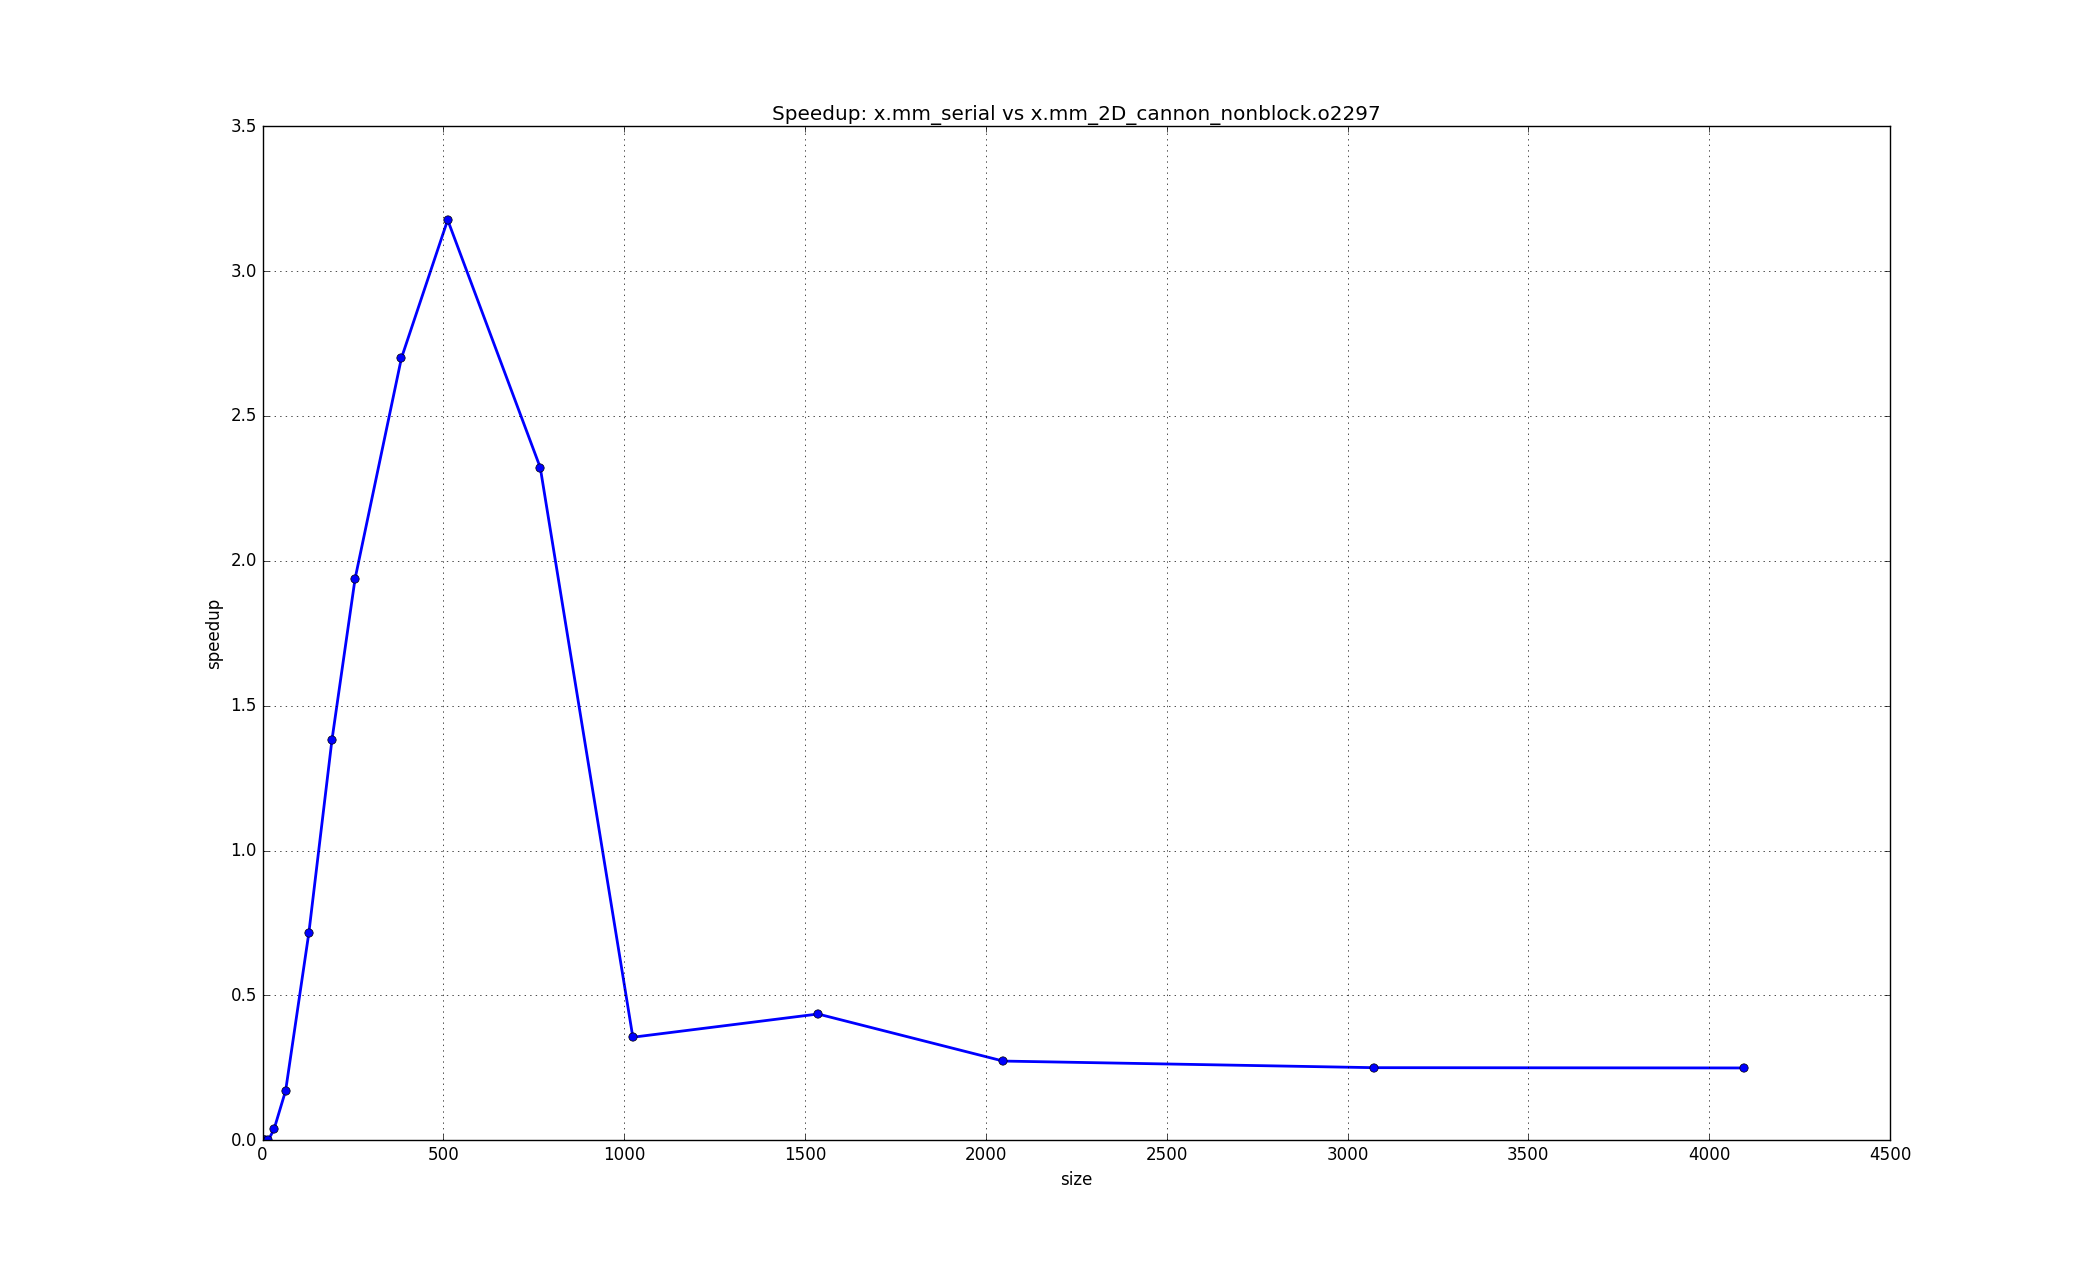
\includegraphics[width=15cm]{immagini/speedup_serial_2d_cannon_nonblock.png}
    \end{center}
    \caption{Speedup seriale vs 2d cannon NON bloccante}
    \label{fig:speedup_serial_2d_cannon_nonblock}
\end{figure}

Come nel precedente caso, lo speedup generale rimane sotto lo 0.5 tranne per le dimensioni che vanno da 192 a 768 dove lo speedup supera il 3. L'efficienza generale \`{e} abbastanza scarsa per tutti quanti gli input: il caso migliore rimane 384 dove l'efficienza raggiunge quasi 0.20. Un valore comunque basso per definire l'implementazione efficiente.

\subsection{MPI con OpenMP}

Per questioni di spazio non verranno riportati i dati grezzi degli esperimenti fatti con OpenMP, ma nell figure \ref{fig:openmp_times} ed \ref{fig:openmp_gflops} si possono vedere le loro rappresentazioni grafiche

\begin{figure}[htbp]
    \begin{center}
        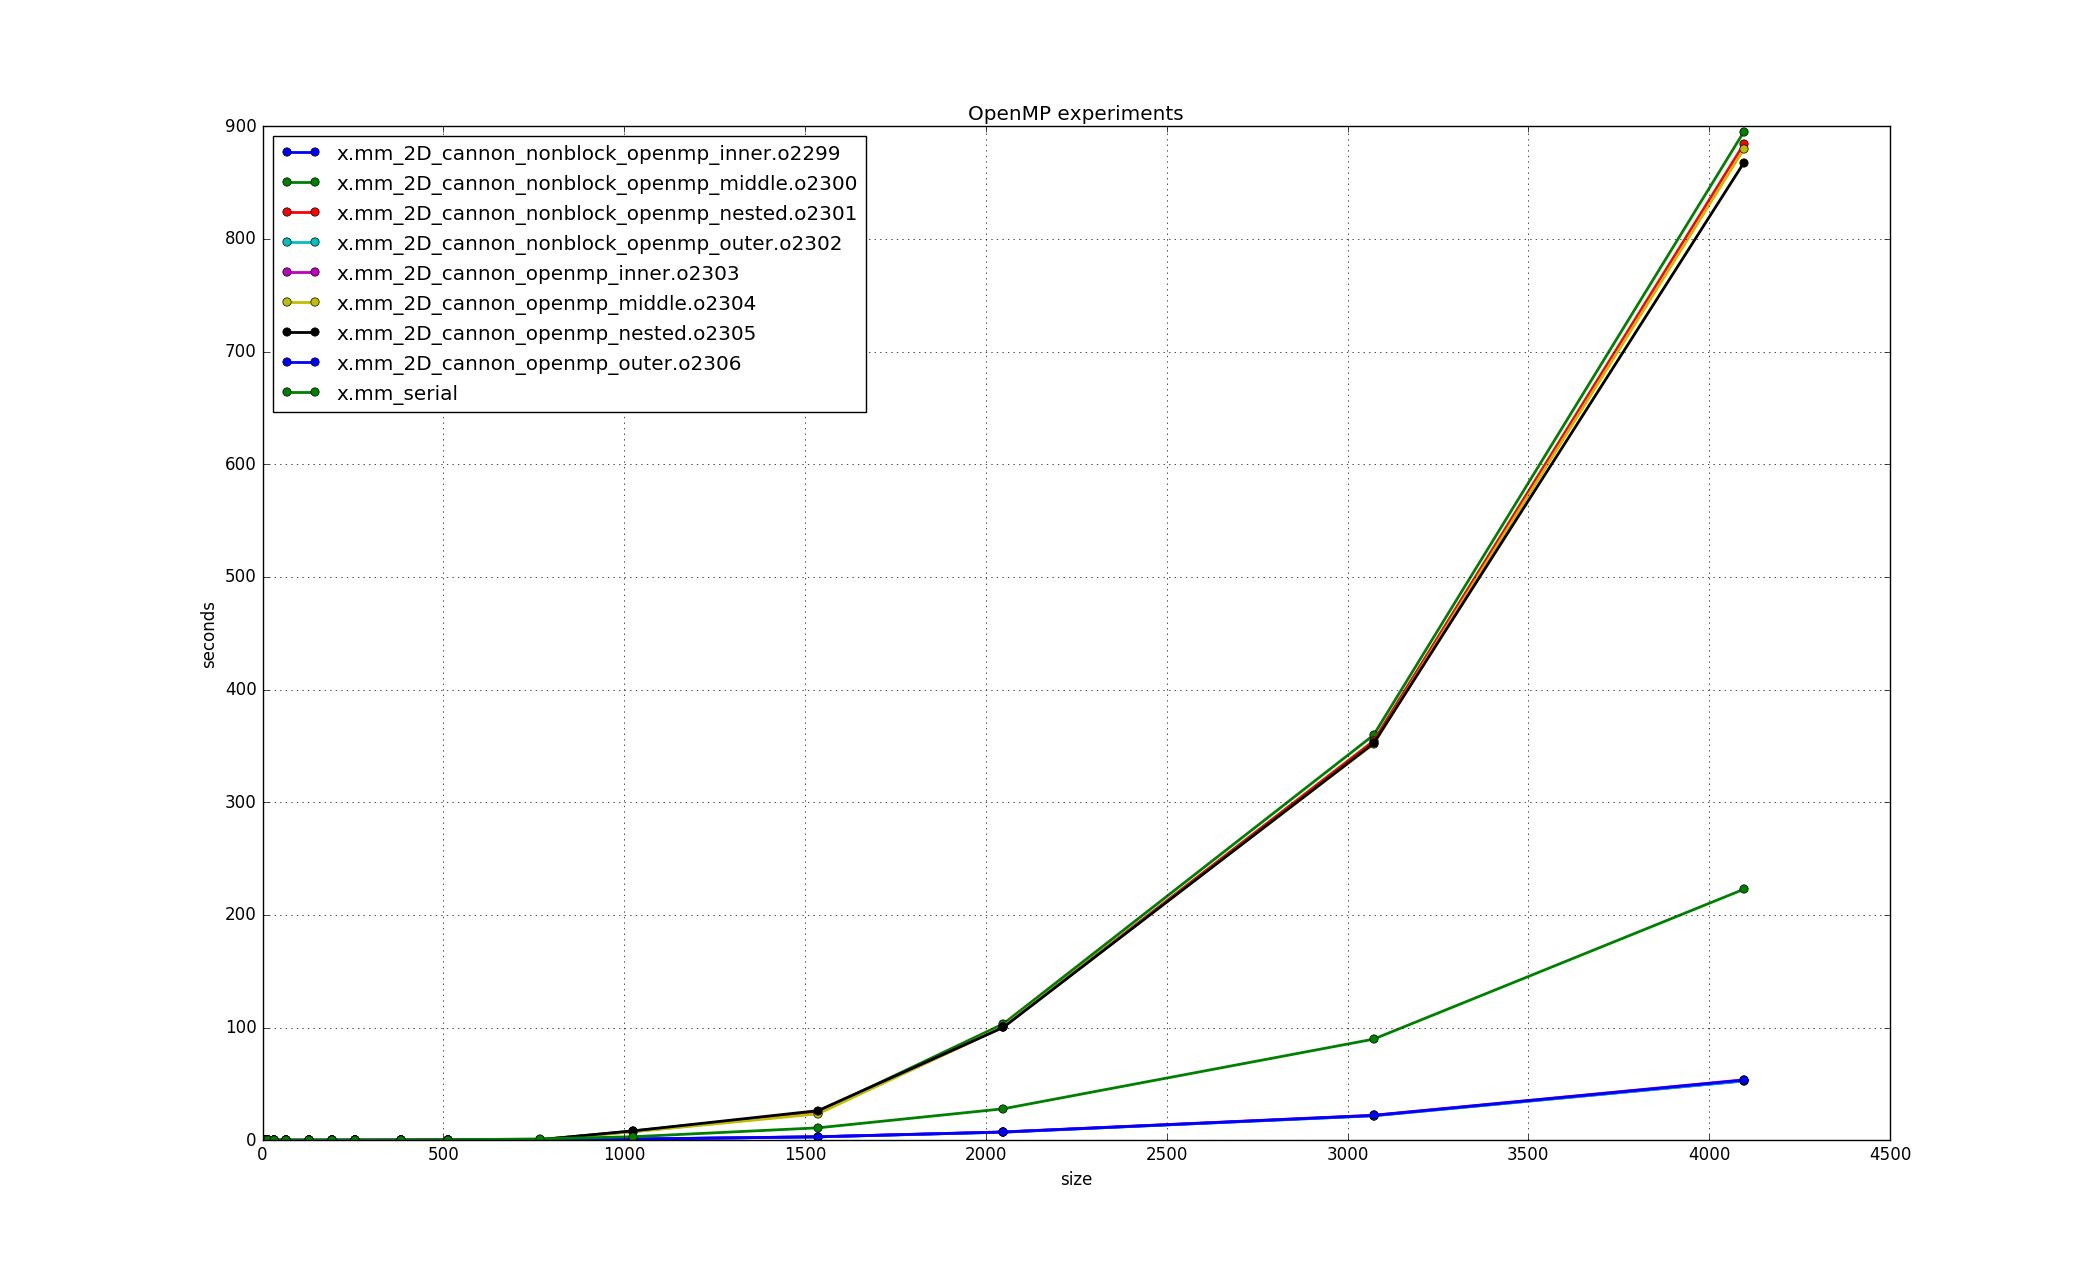
\includegraphics[width=15cm]{immagini/openmp_times.png}
    \end{center}
    \caption{MM MPI with OpenMP: tempo di esecuzione}
    \label{fig:openmp_times}
\end{figure}

\begin{figure}[htbp]
    \begin{center}
        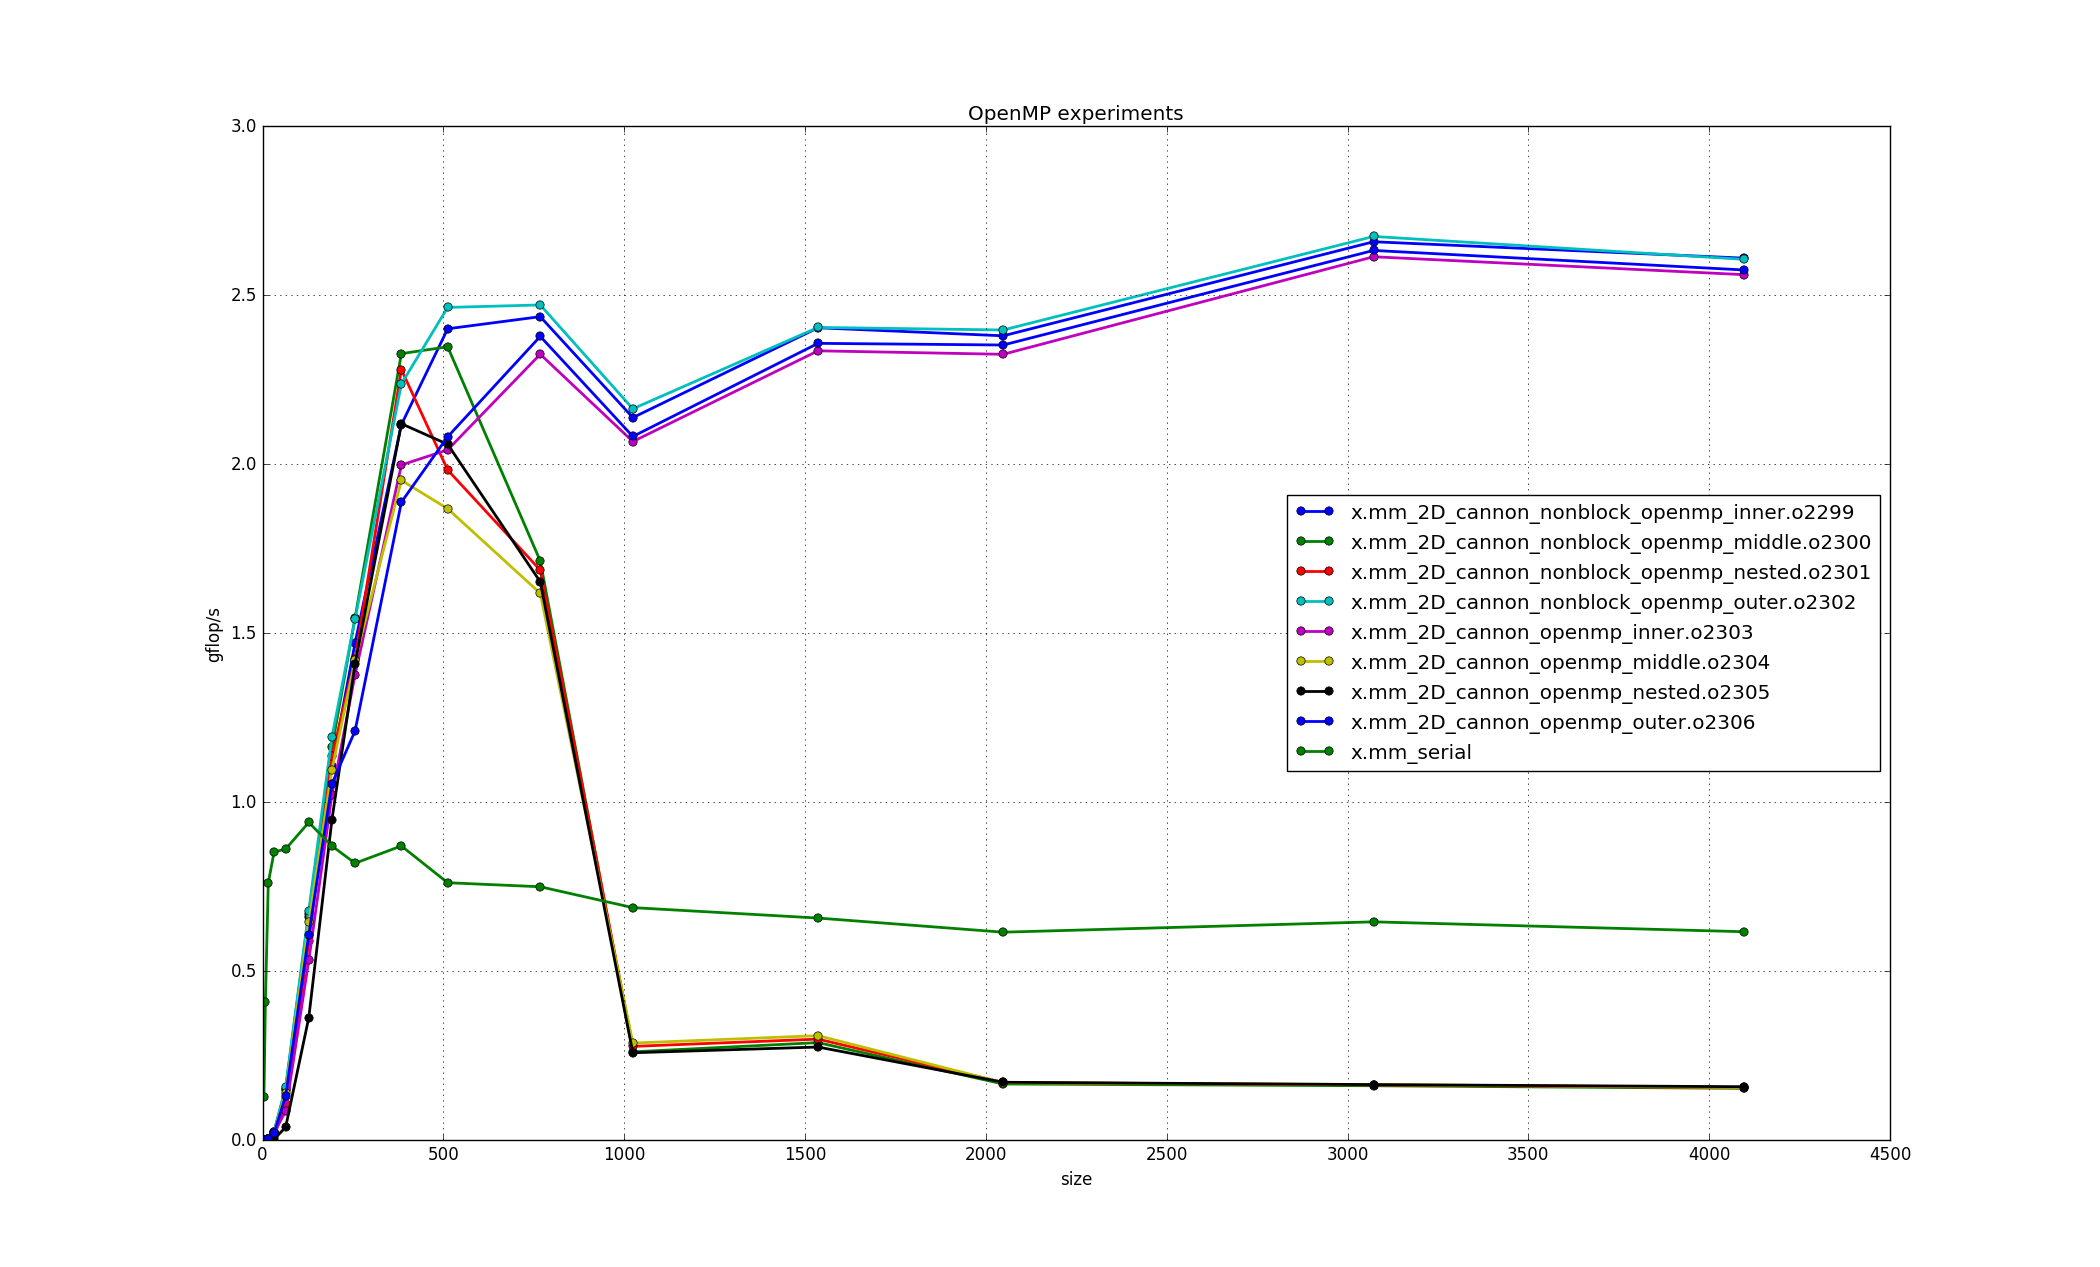
\includegraphics[width=15cm]{immagini/openmp_gflops.png}
    \end{center}
    \caption{MM MPI with OpenMP: Gflop/s}
    \label{fig:openmp_gflops}
\end{figure}

\`{E} interessante vedere come diverse ottimizzazioni OpenMP impattano sulle performance generali dell'algoritmo addirittura rendendo a volte l'algoritmo meno veloce dell'implementazione seriale. Questi sono i casi delle ottimizzazioni middle e nested.
Le ottimizzazioni outer ed inner (sia bloccanti, sia non bloccanti) risultano pi\`{u} veloci dell'implementazione seriale.

\paragraph{Speedup ed efficienza}

Senza calcolare tutti gli speedup e le efficienze di ogni implementazione, si \`{e} scelto di calcolare speedup/efficienza prendendo uno degli algoritmi pi\`{u} veloci: la versione non bloccante con l'ottimizzazione nel ciclo pi\`{u} esterno.

\begin{lstlisting}
size| serial time|  paral time|     speedup|  efficiency
--------------------------------------------------------
   4|         0.0|      0.0019|      0.0000|      0.0000
   8|         0.0|      0.0022|      0.0000|      0.0000
  16|         0.0|      0.0024|      0.0000|      0.0000
  32|      0.0001|      0.0025|      0.0400|      0.0025
  64|      0.0006|      0.0034|      0.1765|      0.0110
 128|      0.0045|      0.0062|      0.7258|      0.0454
 192|      0.0163|      0.0119|      1.3697|      0.0856
 256|      0.0409|      0.0218|      1.8761|      0.1173
 384|      0.1301|      0.0506|      2.5711|      0.1607
 512|      0.3523|      0.1089|      3.2351|      0.2022
 768|       1.208|      0.3666|      3.2951|      0.2059
1024|      3.1203|      0.9924|      3.1442|      0.1965
1536|     11.0251|      3.0139|      3.6581|      0.2286
2048|     27.9096|      7.1668|      3.8943|      0.2434
3072|     89.7327|     21.6833|      4.1383|      0.2586
4096|    222.7798|      52.736|      4.2244|      0.2640
\end{lstlisting}

La figura \ref{fig:speedup_serial_2d_cannon_openmp_outer} mostra il grafico dello speedup tra le due implementazioni.

\begin{figure}[htbp]
    \begin{center}
        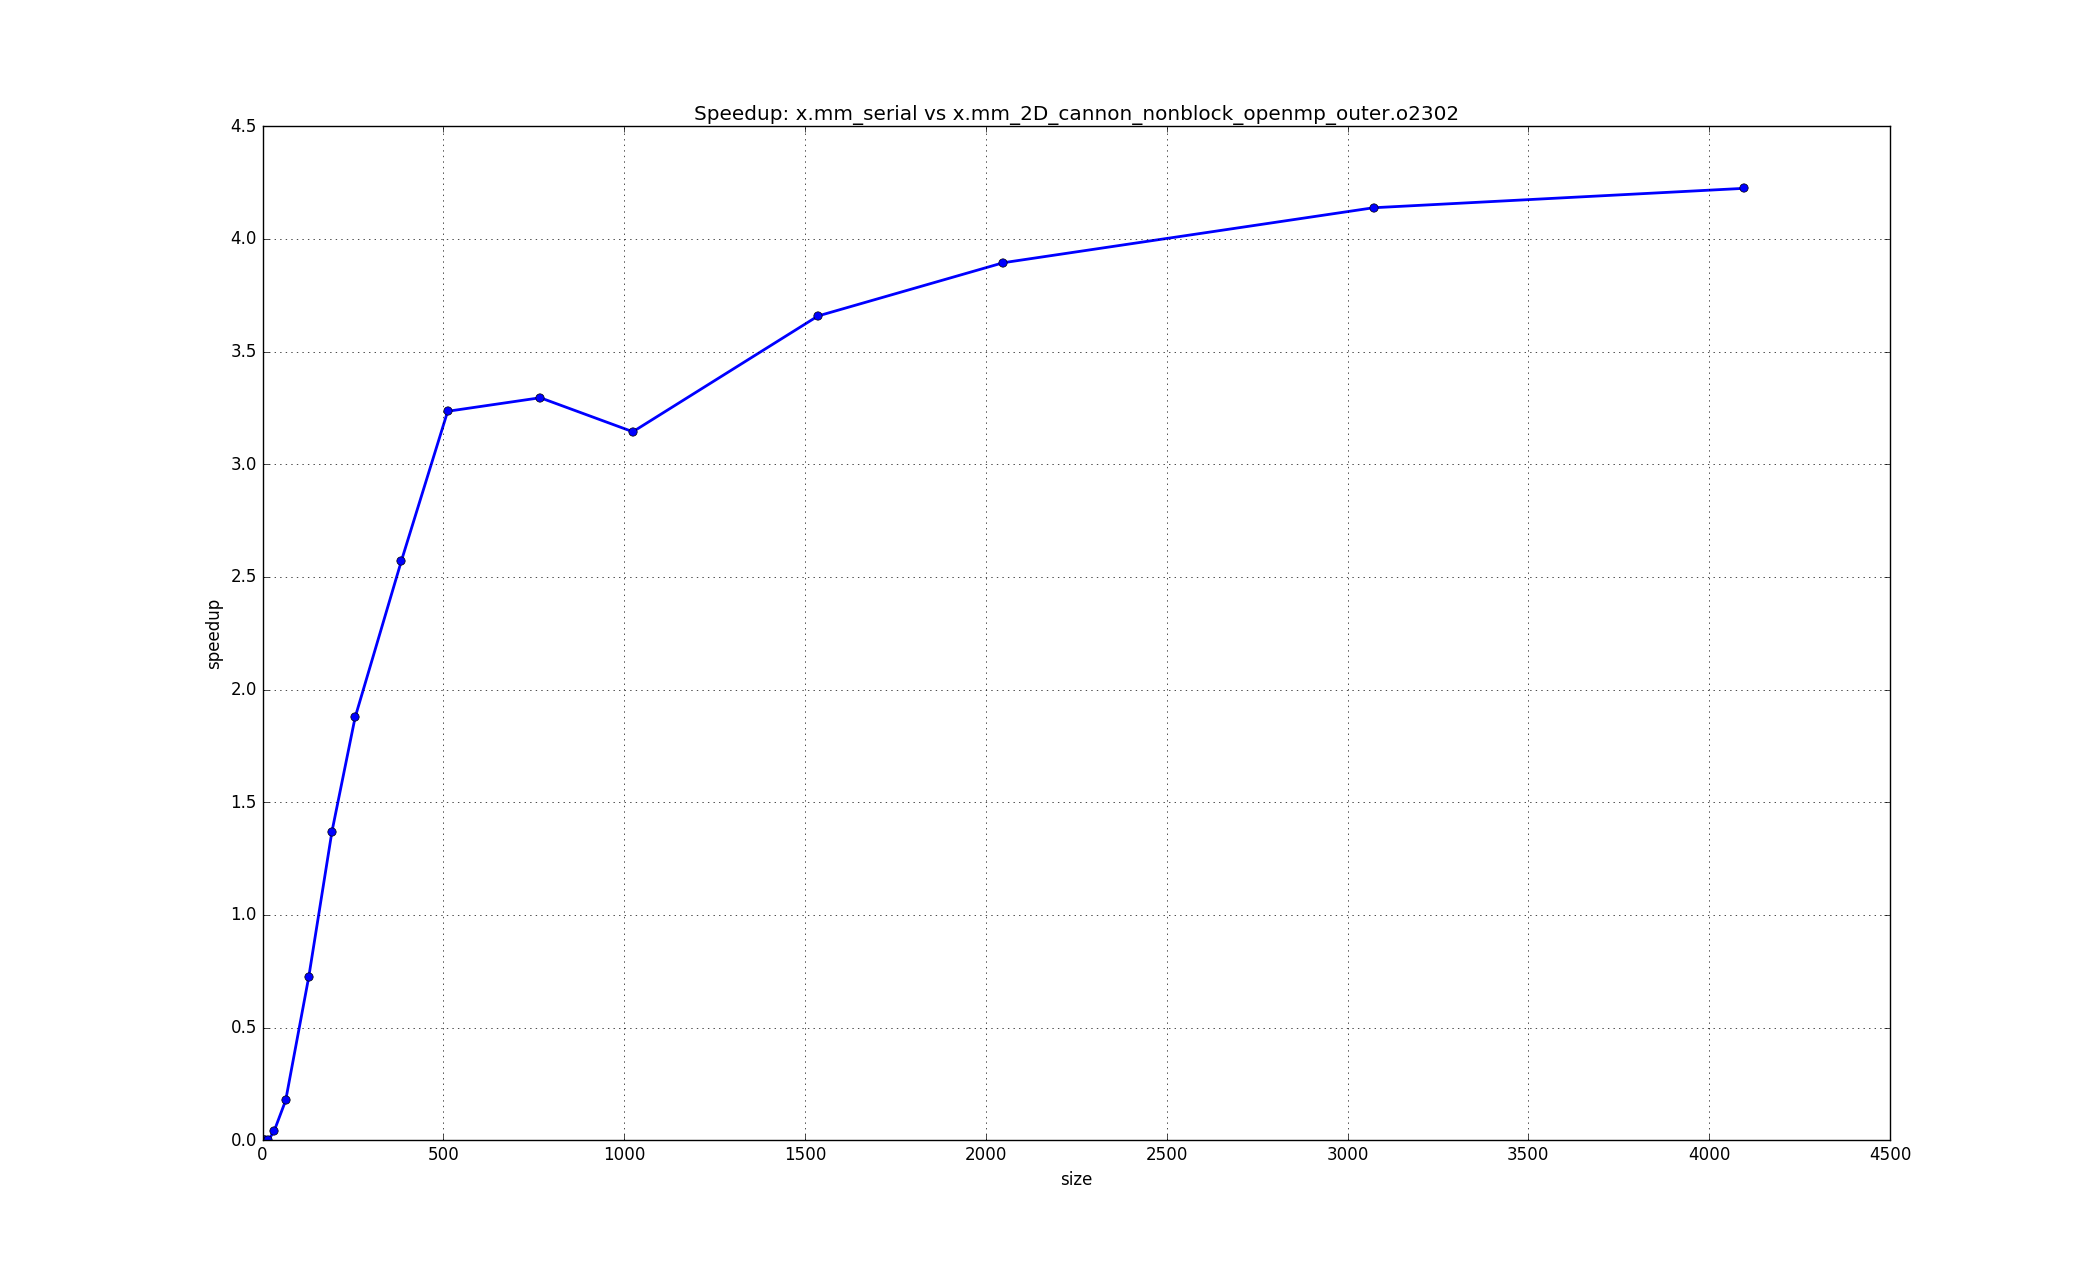
\includegraphics[width=15cm]{immagini/speedup_serial_2d_cannon_openmp_outer.png}
    \end{center}
    \caption{Speedup seriale vs 2d cannon NON bloccante OpenMP outer}
    \label{fig:speedup_serial_2d_cannon_openmp_outer}
\end{figure}

Come si pu\`{o} vedere sia dai dati sia dall figura \ref{fig:speedup_serial_2d_cannon_openmp_outer}, lo speedup inizia ad essere migliore rispetto alle precedenti implementazioni. Infatto si arriva ad avere uno speedup di 4 per le dimensioni pi\`{u} grandi (3072, 4096). Di conseguenza anche l'efficienza ha un massimo di circa 0.27, poco pi\`{u} di un quarto dell'efficienza ideale (1).
Questa implementazione inizia ad essere pi\`{u} interessante soprattuto per dimensioni pi\`{u} grandi dove una potenza di calcolo distribuito diventa una necessit\`{a}.

\subsection{MPI con CBLAS}

Come nel caso precedente, non si riportano i dati grezzi degli esperimenti fatti con l'ottimizzazione CBLAS ma le figure \ref{fig:cblas_times} e \ref{fig:cblas_gflops} rappresentano in maniera esaustiva i risultati di questi esperimenti.

\begin{figure}[htbp]
    \begin{center}
        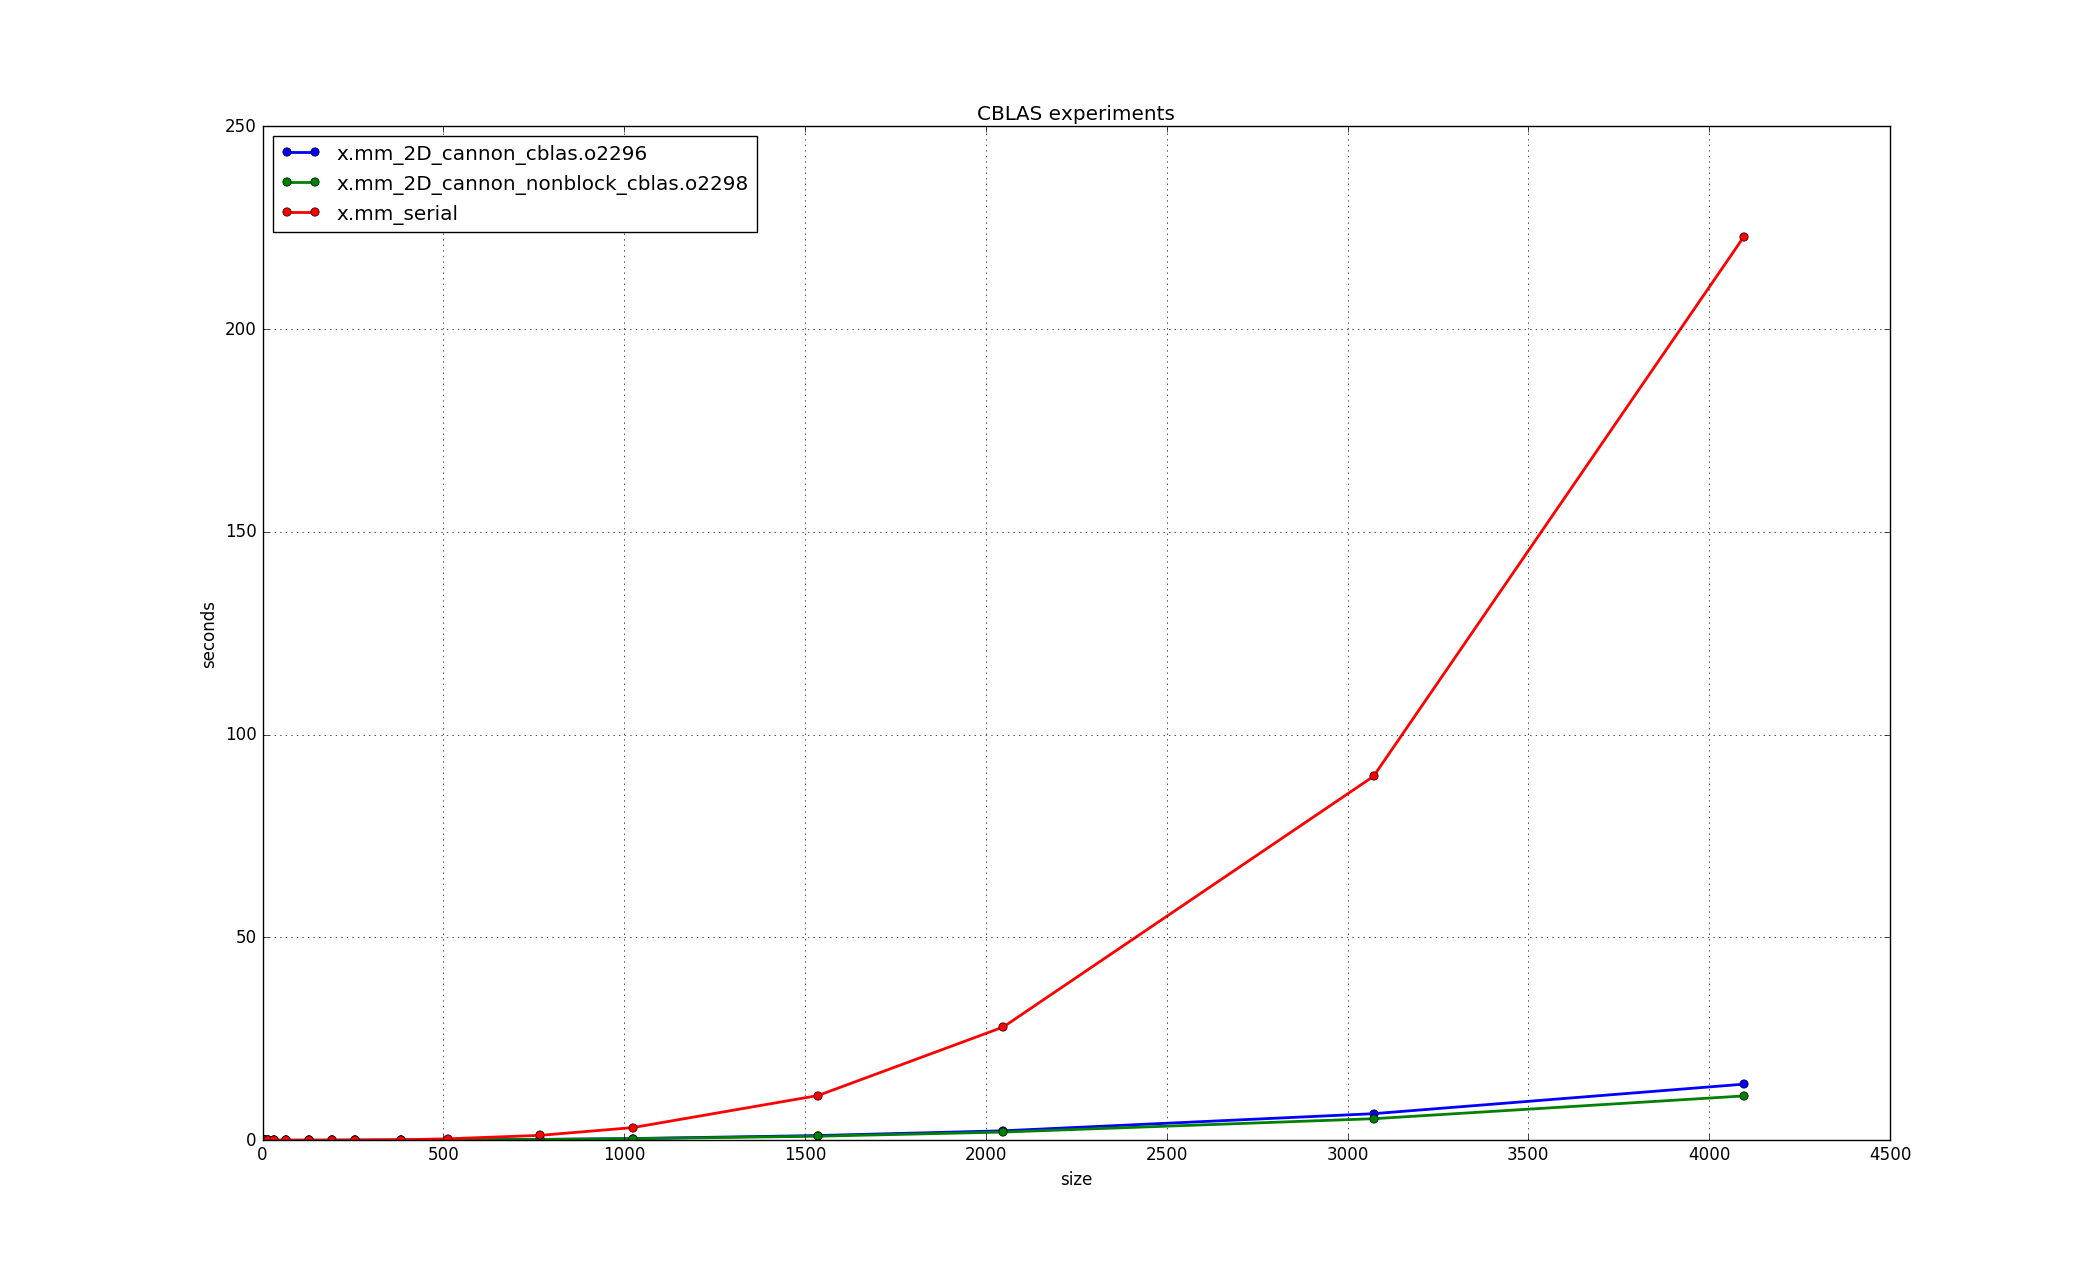
\includegraphics[width=15cm]{immagini/cblas_times.png}
    \end{center}
    \caption{MM MPI with CBLAS: tempo di esecuzione}
    \label{fig:cblas_times}
\end{figure}

\begin{figure}[htbp]
    \begin{center}
        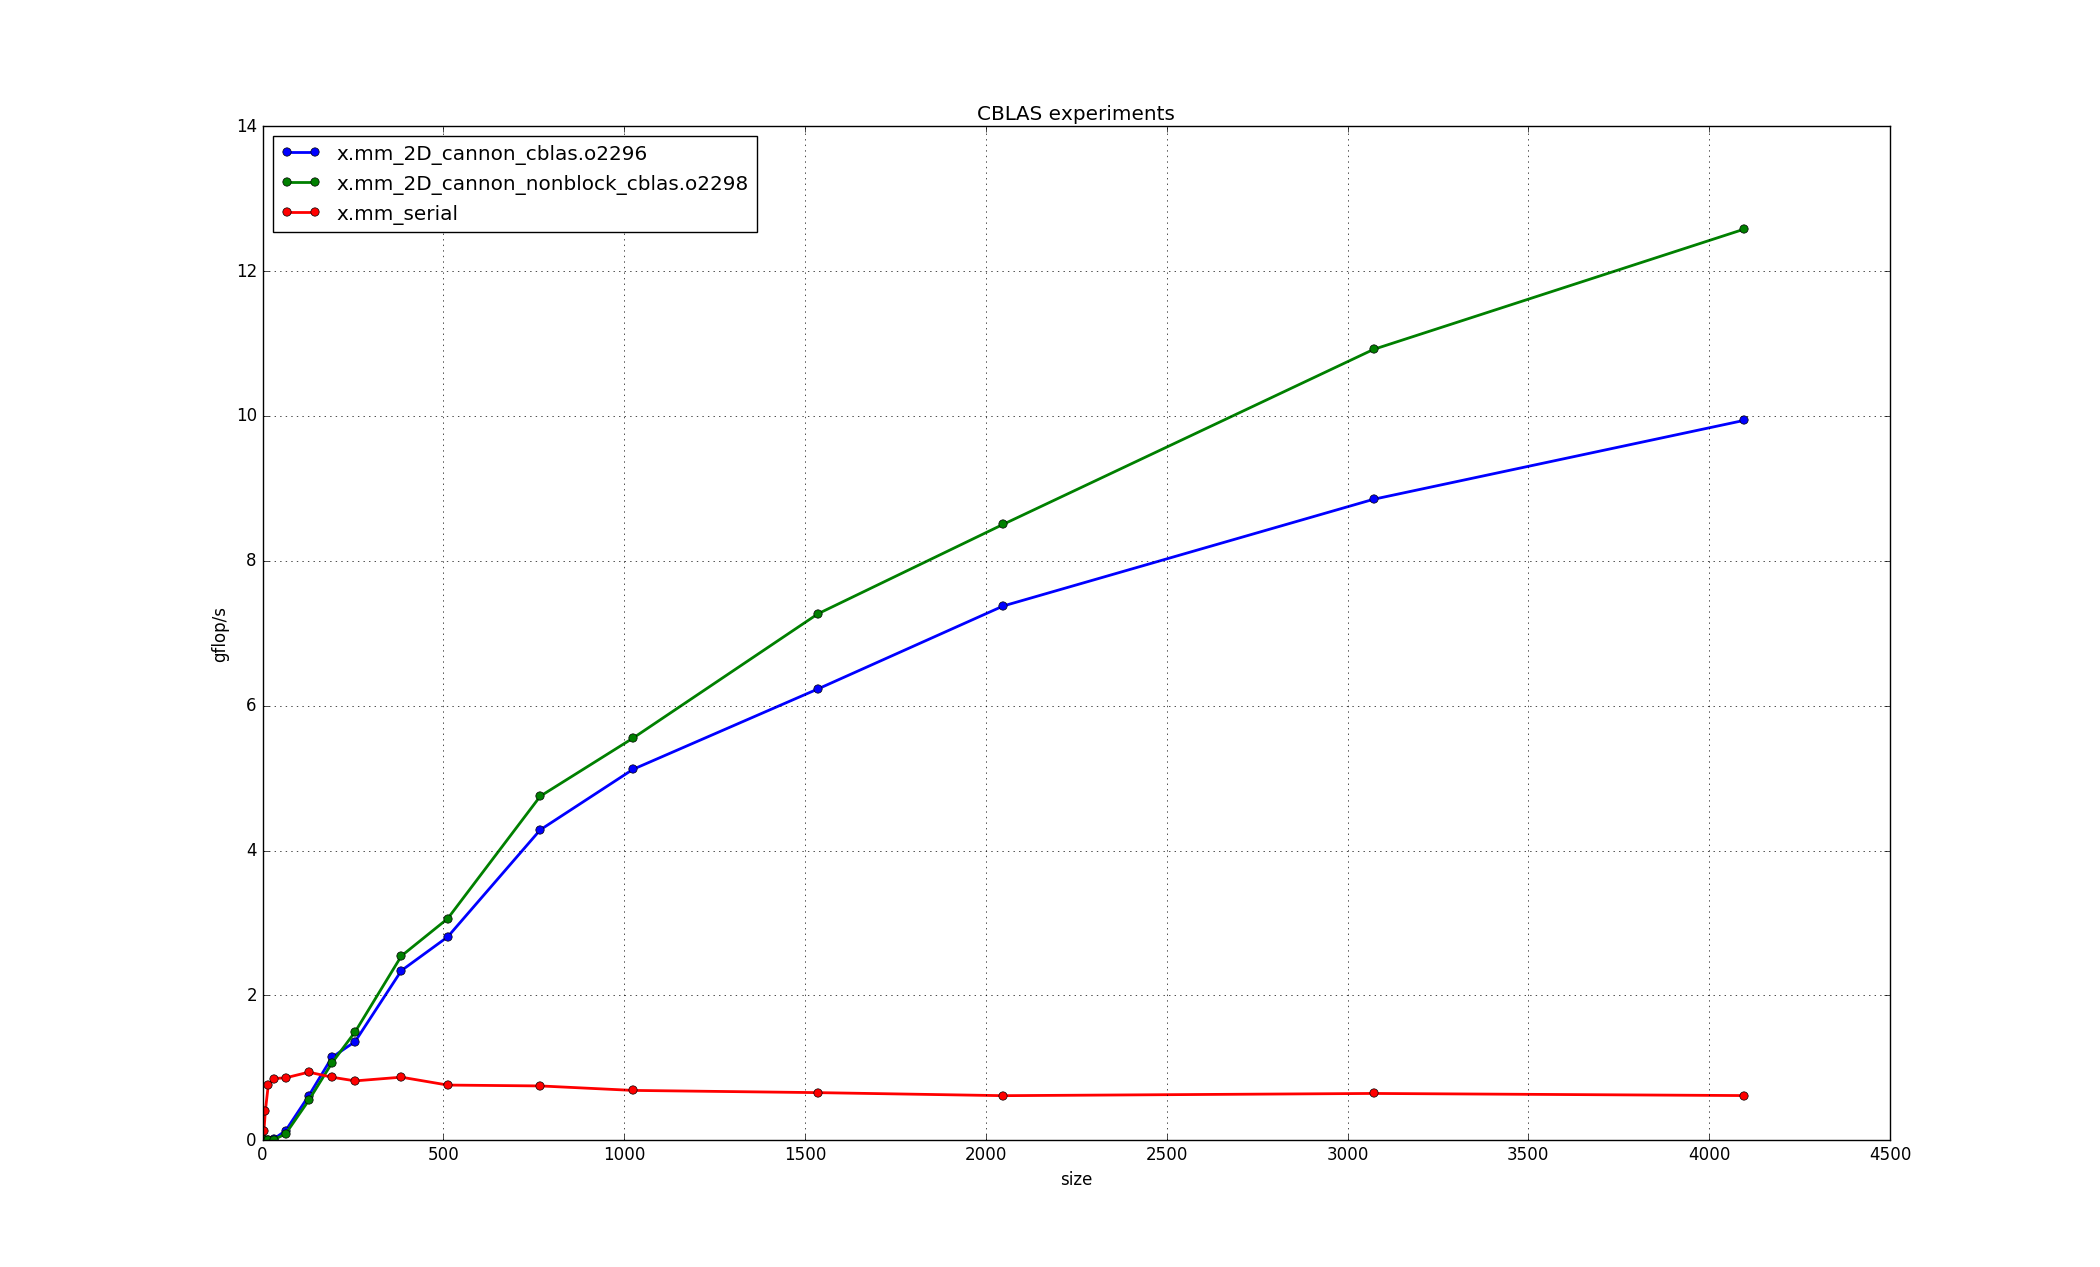
\includegraphics[width=15cm]{immagini/cblas_gflops.png}
    \end{center}
    \caption{MM MPI with CBLAS: Gflop/s}
    \label{fig:cblas_gflops}
\end{figure}

Con l'ottimizzazione cblas si nota subito un netto miglioramento di velocit\`{a} e throughput, portando la versione non bloccante in leggero vantaggio rispetto alla corrispettiva bloccante. Questo significa che l'utilizzo di primitive non bloccanti ottimizza l'uso delle risorse evitando momenti "morti" che potrebbero essere utilizzati per effettuare la moltiplicazione.

\paragraph{Speedup ed efficienza}

Dunque l'implementazione cblas pi\`{u} veloce \`{e} quella non bloccante: i risultati di questa verranno utilizzati per calcolare speedup ed efficienza.

\begin{lstlisting}
size| serial time|  paral time|     speedup|  efficiency
--------------------------------------------------------
   4|         0.0|      0.0018|      0.0000|      0.0000
   8|         0.0|      0.0217|      0.0000|      0.0000
  16|         0.0|      0.0124|      0.0000|      0.0000
  32|      0.0001|      0.0076|      0.0132|      0.0008
  64|      0.0006|      0.0059|      0.1017|      0.0064
 128|      0.0045|      0.0076|      0.5921|      0.0370
 192|      0.0163|      0.0133|      1.2256|      0.0766
 256|      0.0409|      0.0224|      1.8259|      0.1141
 384|      0.1301|      0.0445|      2.9236|      0.1827
 512|      0.3523|      0.0877|      4.0171|      0.2511
 768|       1.208|      0.1907|      6.3346|      0.3959
1024|      3.1203|      0.3869|      8.0649|      0.5041
1536|     11.0251|      0.9971|     11.0572|      0.6911
2048|     27.9096|      2.0202|     13.8153|      0.8635
3072|     89.7327|      5.3102|     16.8982|      1.0561
4096|    222.7798|     10.9267|     20.3886|      1.2743
\end{lstlisting}

La figura \ref{fig:speedup_serial_2d_cannon_nonblock_cblas} mostra il grafico dello speedup tra le due implementazioni.

\begin{figure}[htbp]
    \begin{center}
        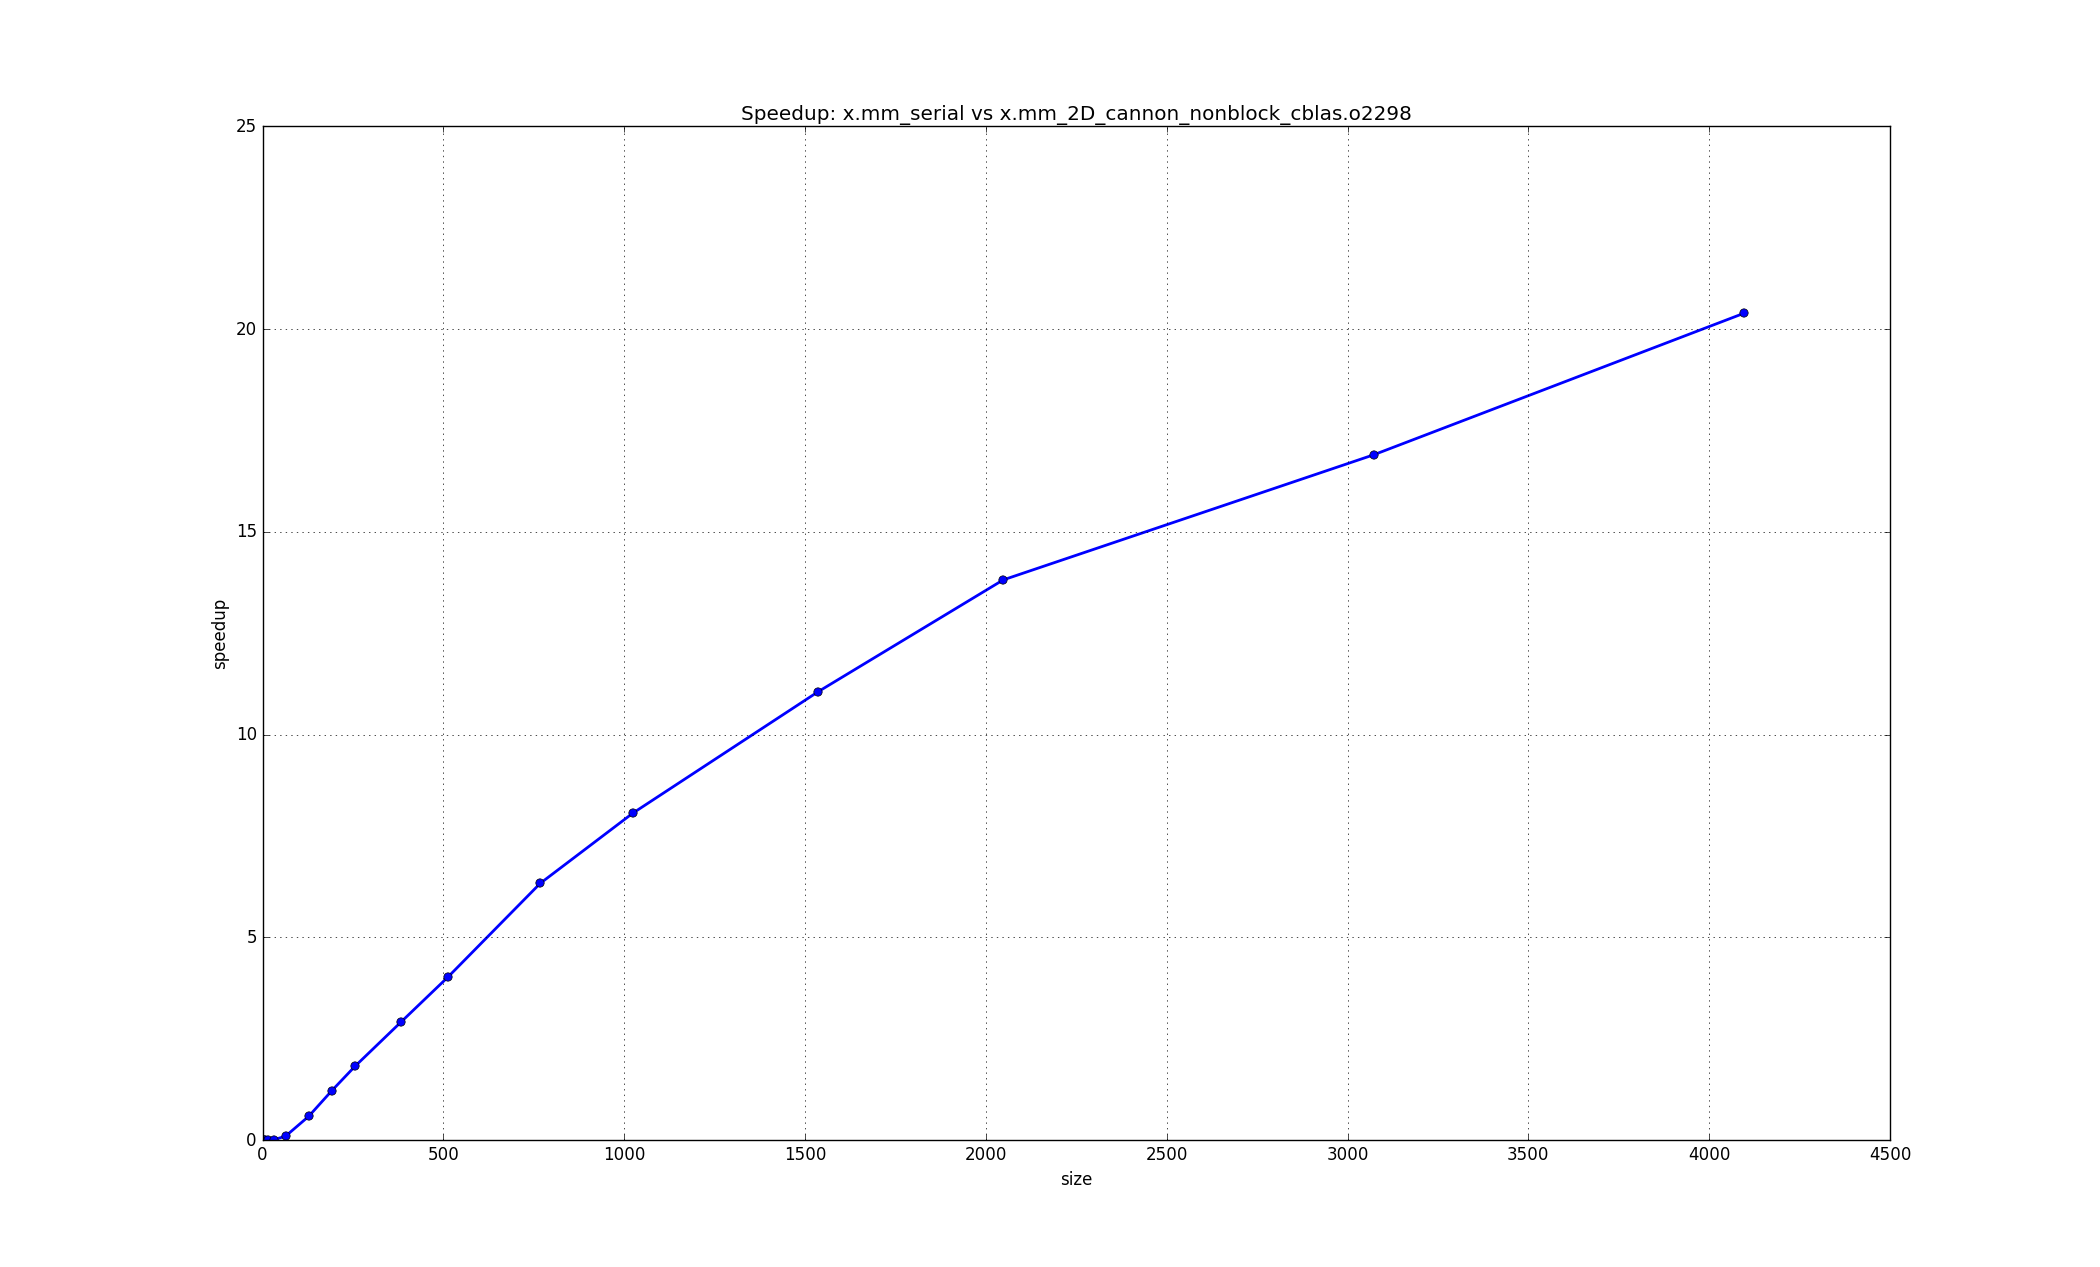
\includegraphics[width=15cm]{immagini/speedup_serial_2d_cannon_nonblock_cblas.png}
    \end{center}
    \caption{Speedup seriale vs 2d cannon NON bloccante CBLAS}
    \label{fig:speedup_serial_2d_cannon_nonblock_cblas}
\end{figure}

Questa \`{e} la migliore implementazione in assoluto: infatti a partire dalla dimensione 3072 inizia ad avere uno speedup ed una efficienza maggiori di quella ideale.
Si ricorda che lo speedup ideale equivale a $S_{ideale}(p) = p$ mentre l'efficienza ideale equivale a $E_{ideale}(p) = 1$.
Dunque per matrici medio grandi, l'implementazione non bloccante con cblas \`{e} pi\`{u} che ideale.


\subsection{Visioni di insieme}
In questa ultima sezione si ha una visione di insieme su tutti esperimenti effettuati (figure \ref{fig:all_times} e \ref{fig:all_gflops}).

\begin{figure}[htbp]
    \begin{center}
        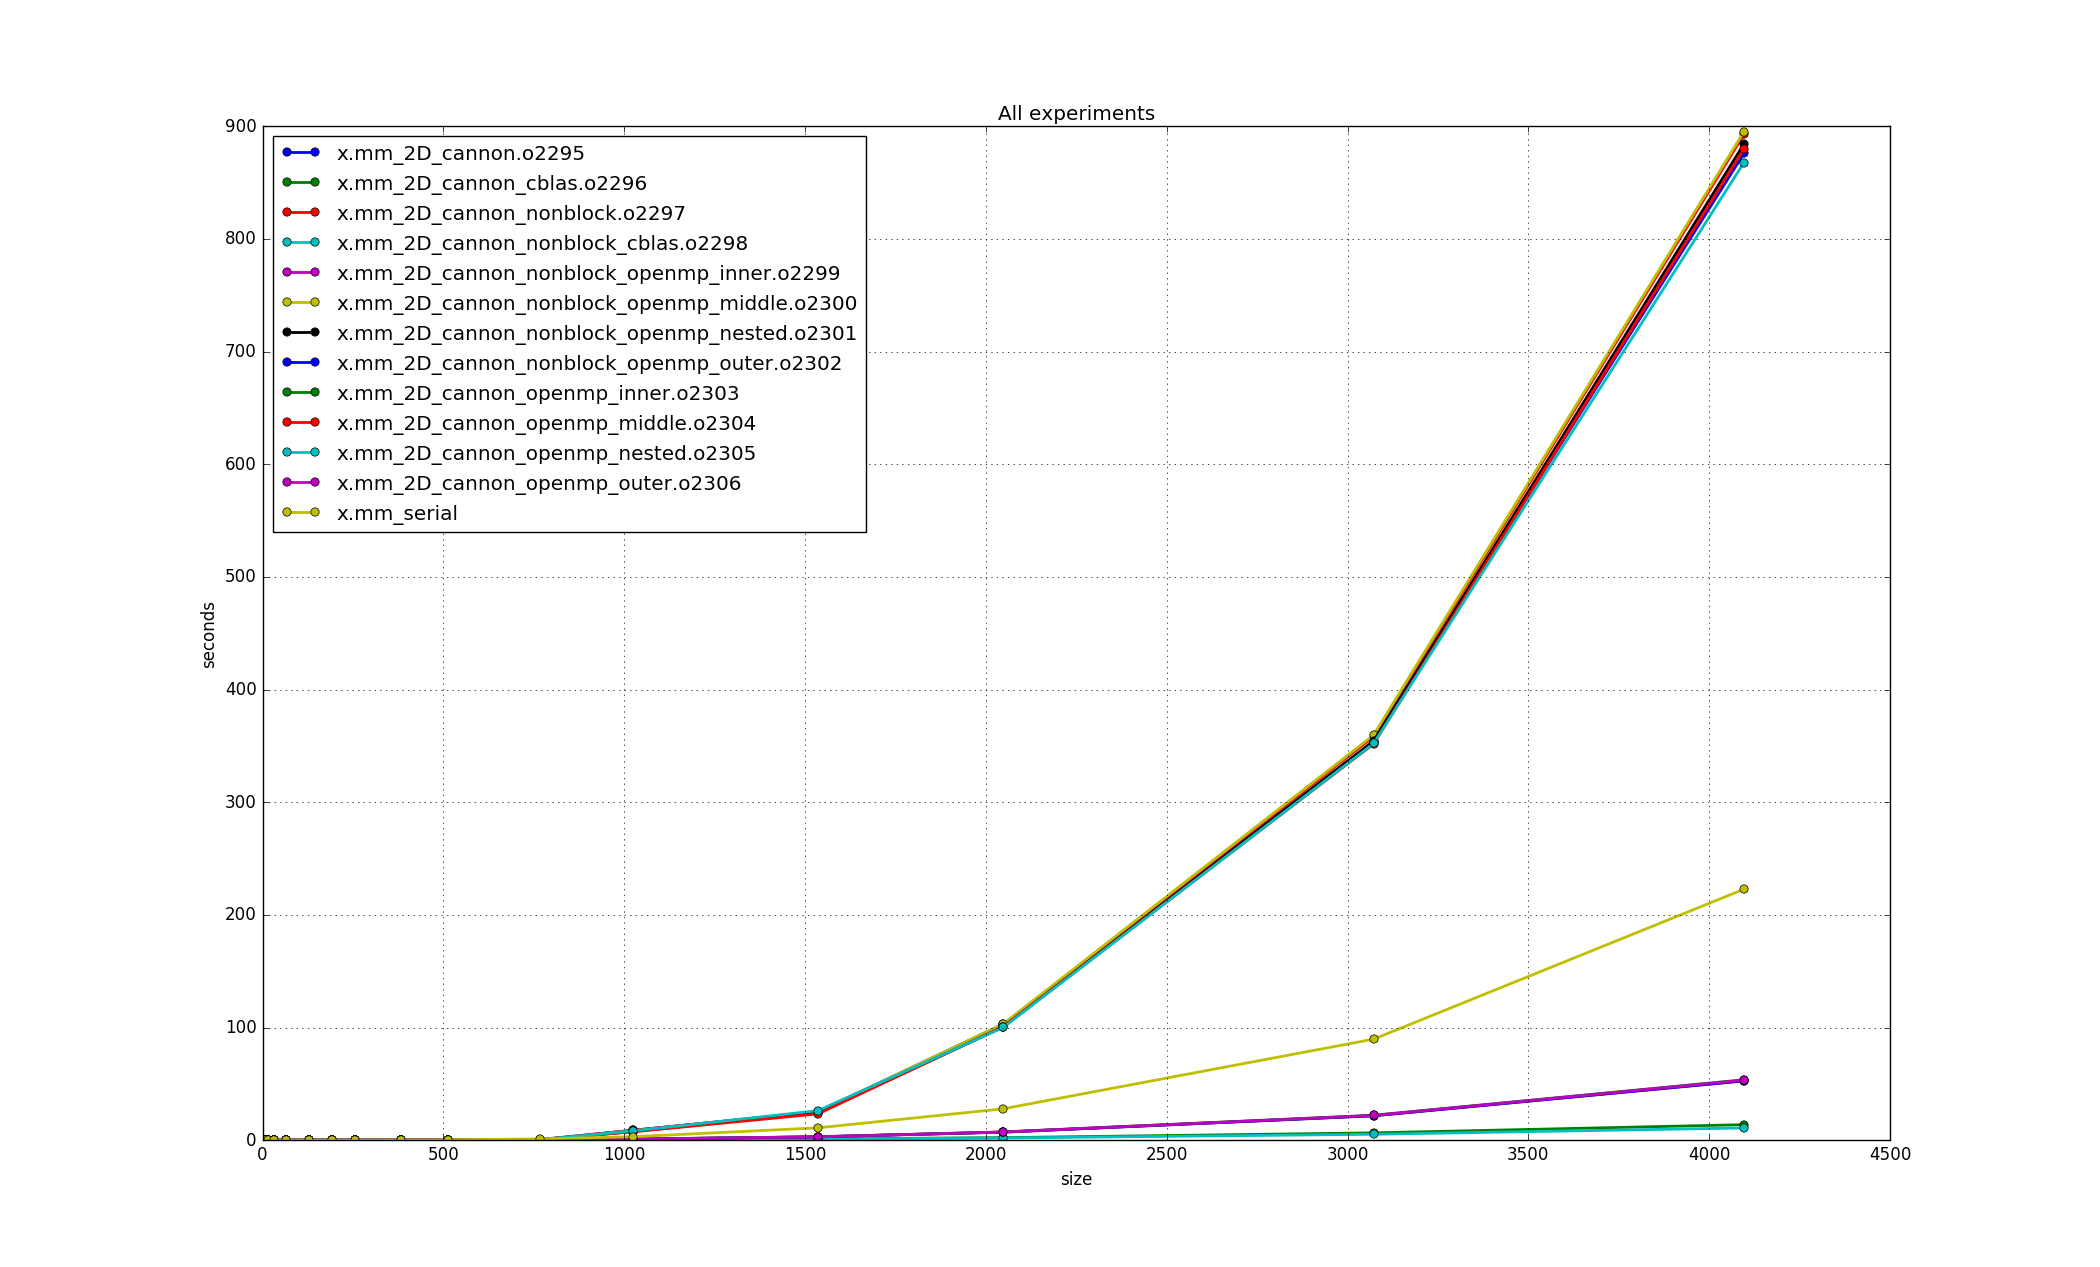
\includegraphics[width=15cm]{immagini/all_times.png}
    \end{center}
    \caption{MM MPI: tempo di esecuzione}
    \label{fig:all_times}
\end{figure}

\begin{figure}[htbp]
    \begin{center}
        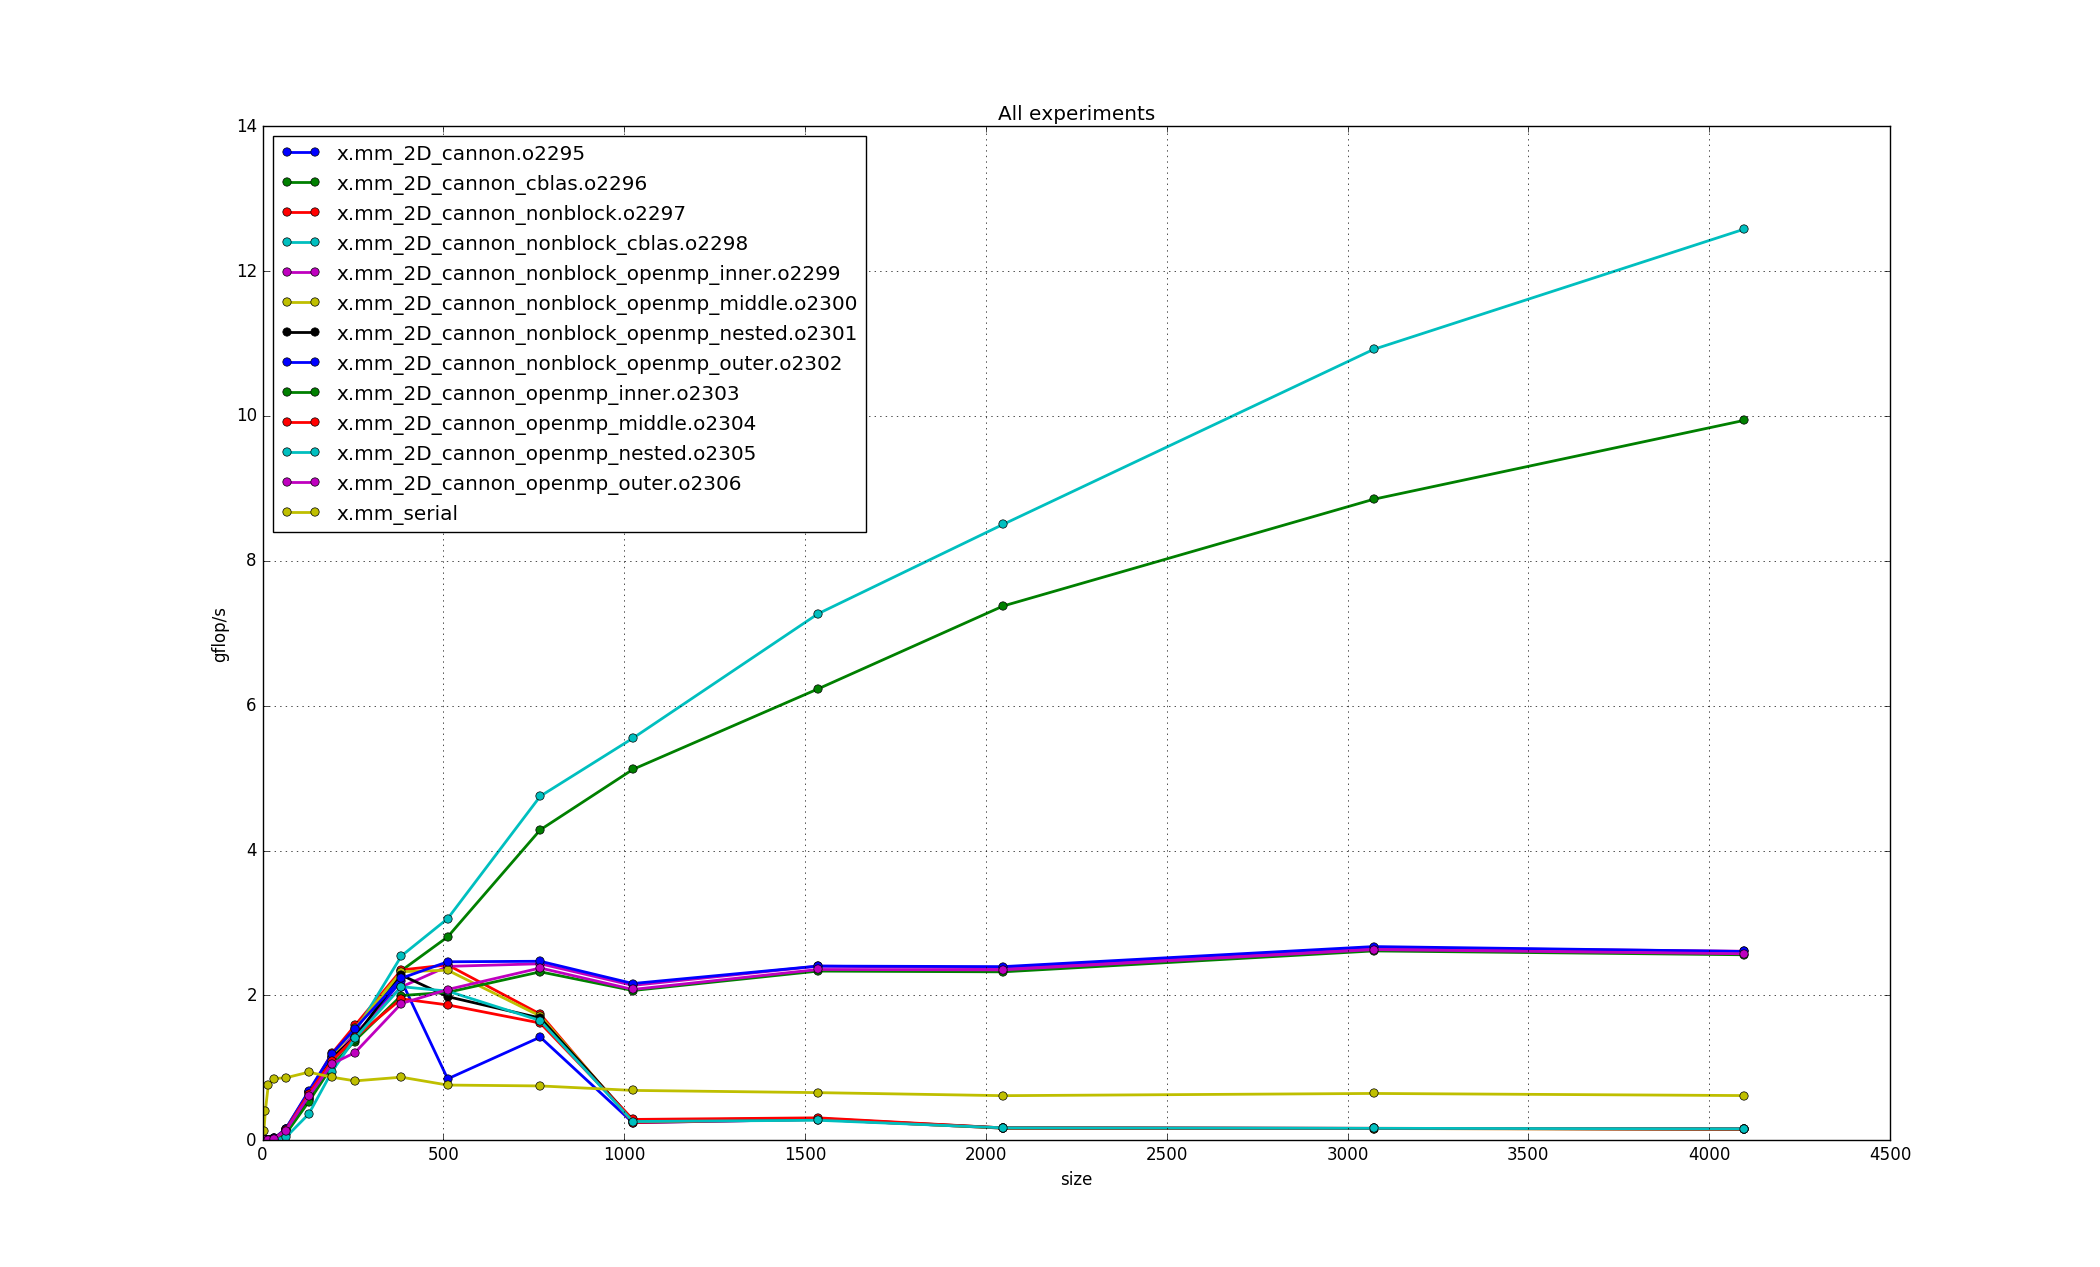
\includegraphics[width=15cm]{immagini/all_gflops.png}
    \end{center}
    \caption{MM MPI: Gflop/s}
    \label{fig:all_gflops}
\end{figure}

Tutti gli esperimenti bloccanti nelle figure \ref{fig:blocking_times} e \ref{fig:blocking_gflops}

\begin{figure}[htbp]
    \begin{center}
        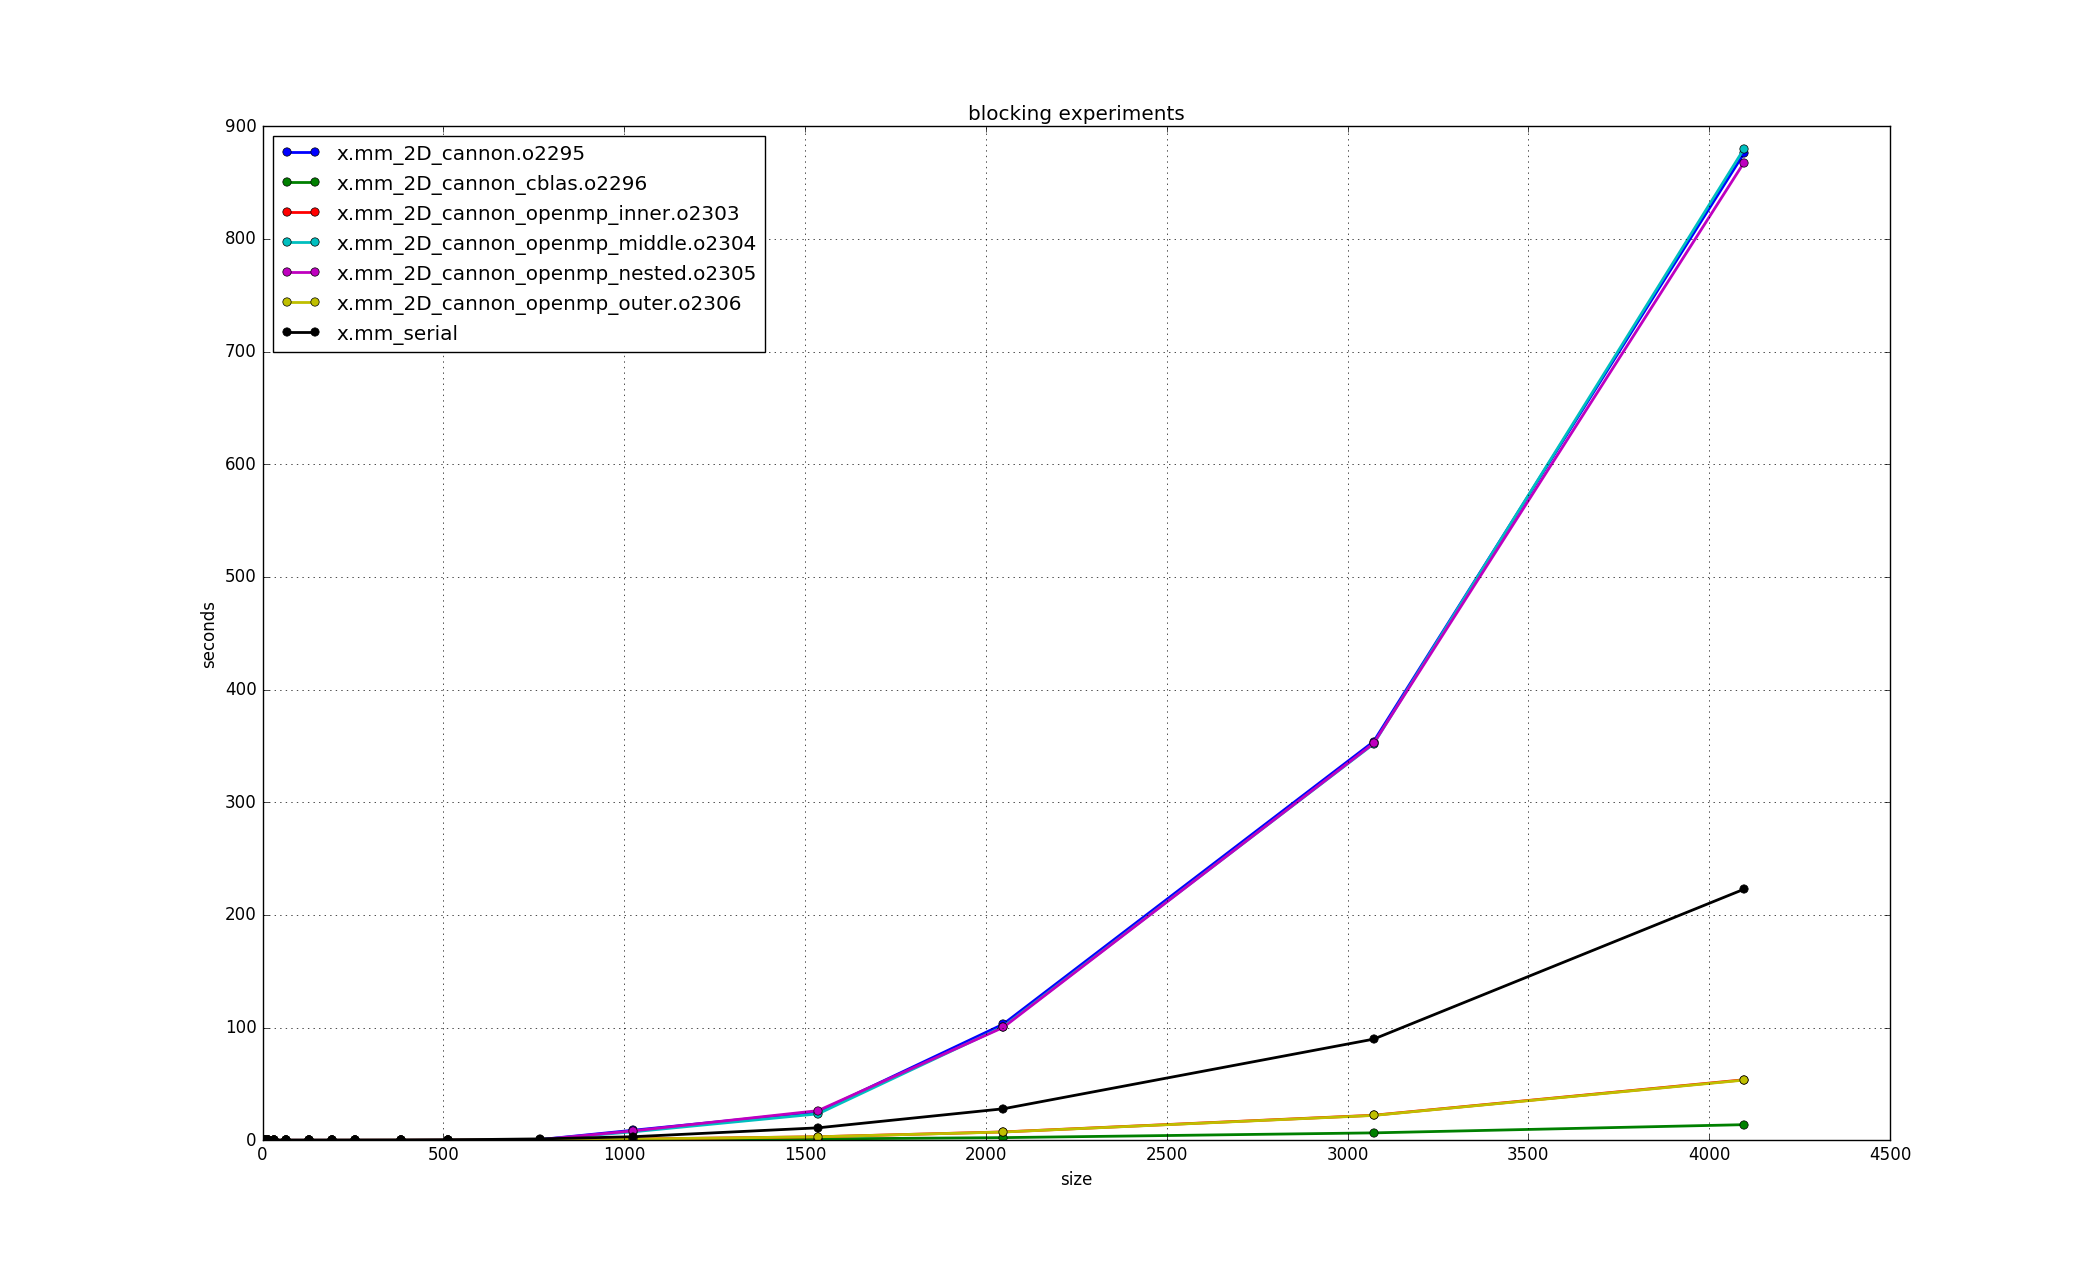
\includegraphics[width=15cm]{immagini/blocking_times.png}
    \end{center}
    \caption{MM MPI bloccanti: tempo di esecuzione}
    \label{fig:blocking_times}
\end{figure}

\begin{figure}[htbp]
    \begin{center}
        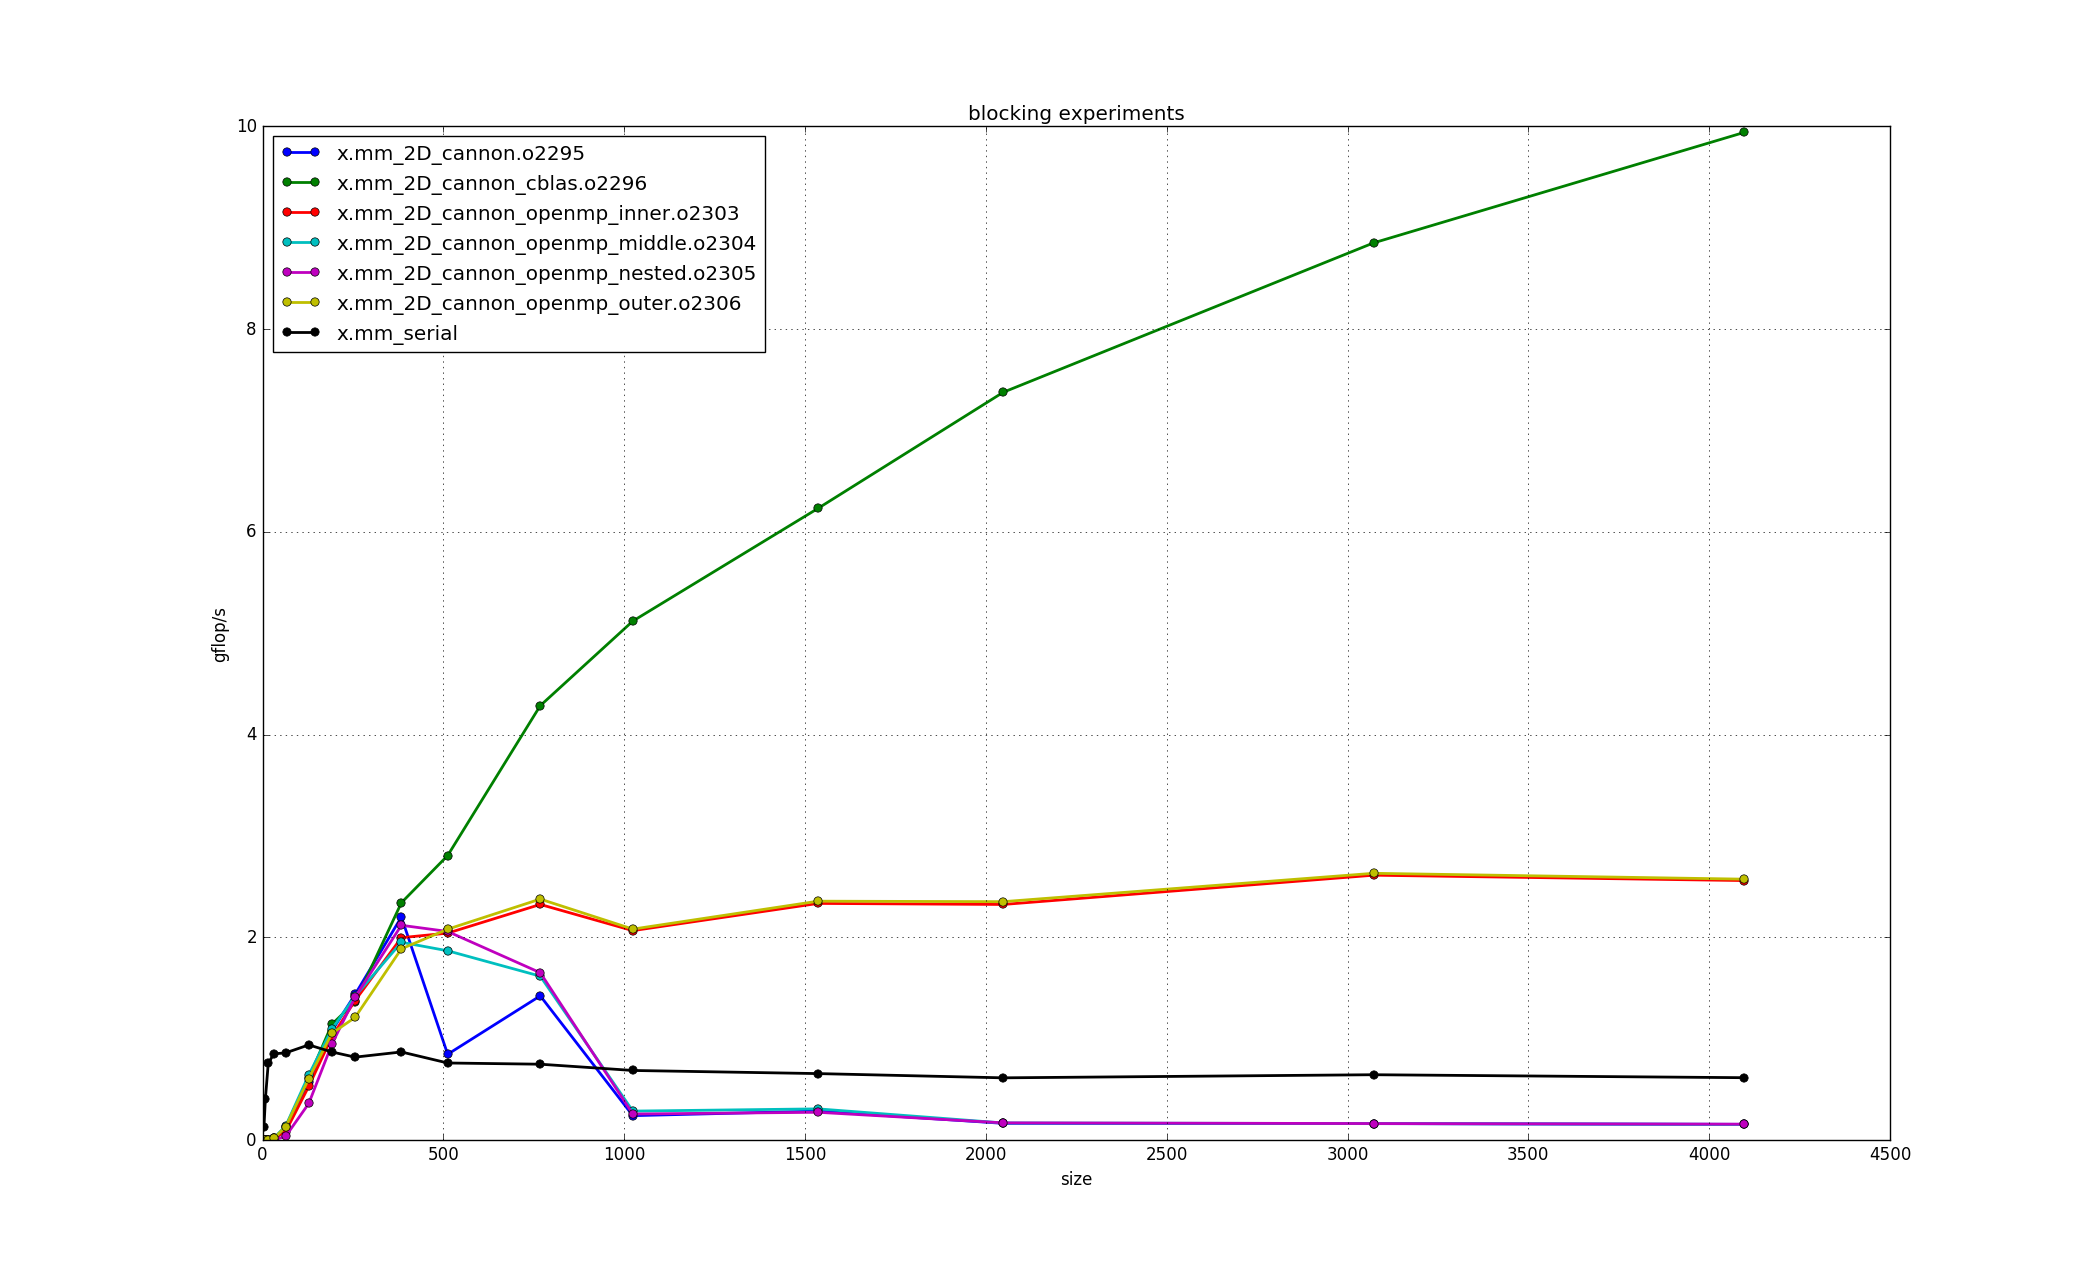
\includegraphics[width=15cm]{immagini/blocking_gflops.png}
    \end{center}
    \caption{MM MPI bloccanti: Gflop/s}
    \label{fig:blocking_gflops}
\end{figure}

Tutti gli esperimenti NON bloccanti nelle figure \ref{fig:non_blocking_times} e \ref{fig:non_blocking_gflops}

\begin{figure}[htbp]
    \begin{center}
        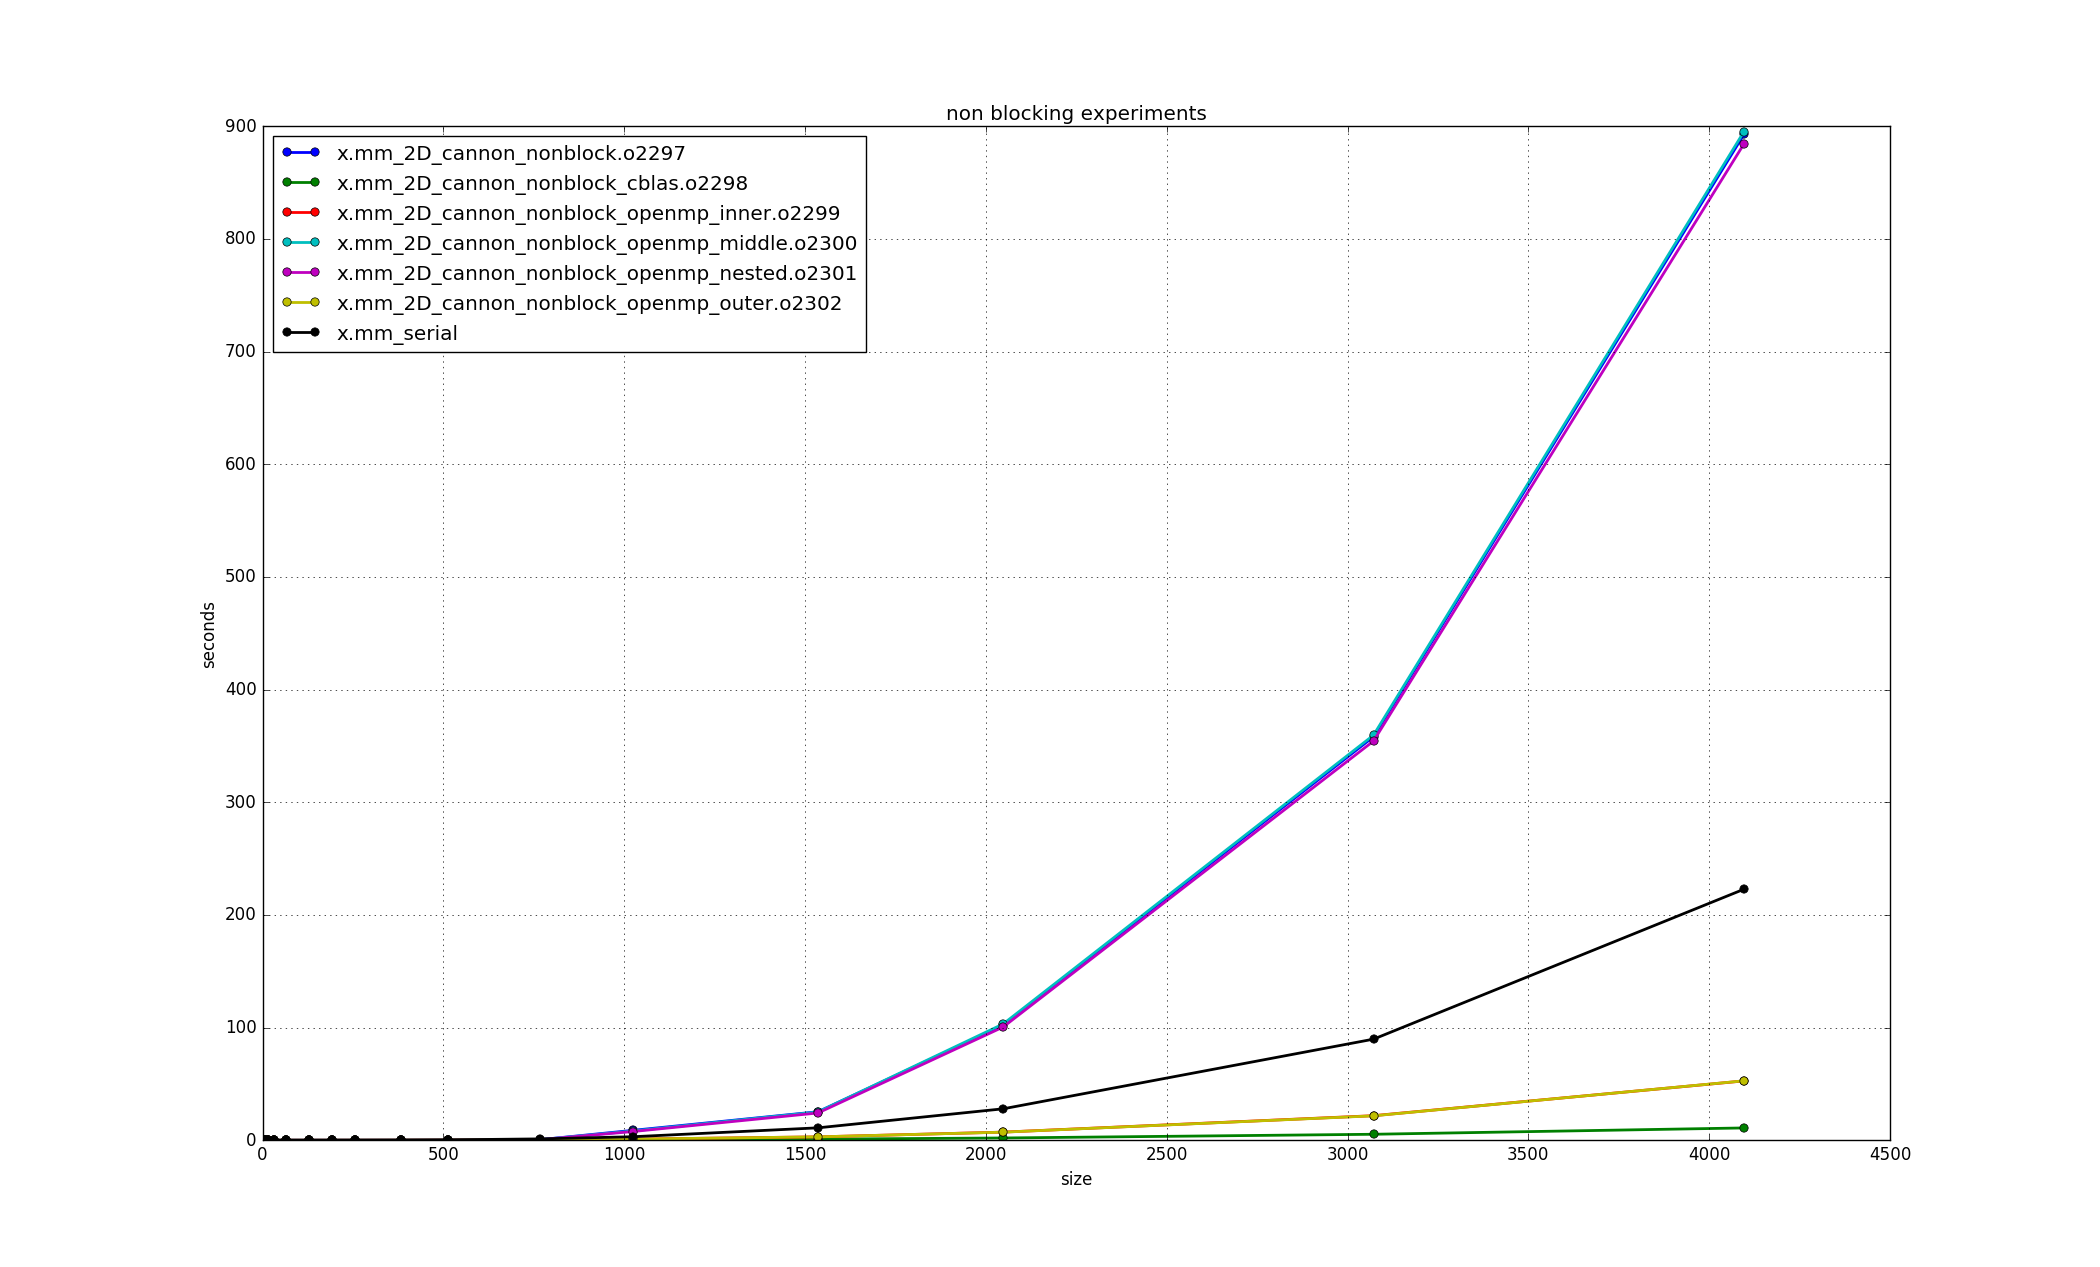
\includegraphics[width=15cm]{immagini/non_blocking_times.png}
    \end{center}
    \caption{MM MPI NON bloccanti: tempo di esecuzione}
    \label{fig:non_blocking_times}
\end{figure}

\begin{figure}[htbp]
    \begin{center}
        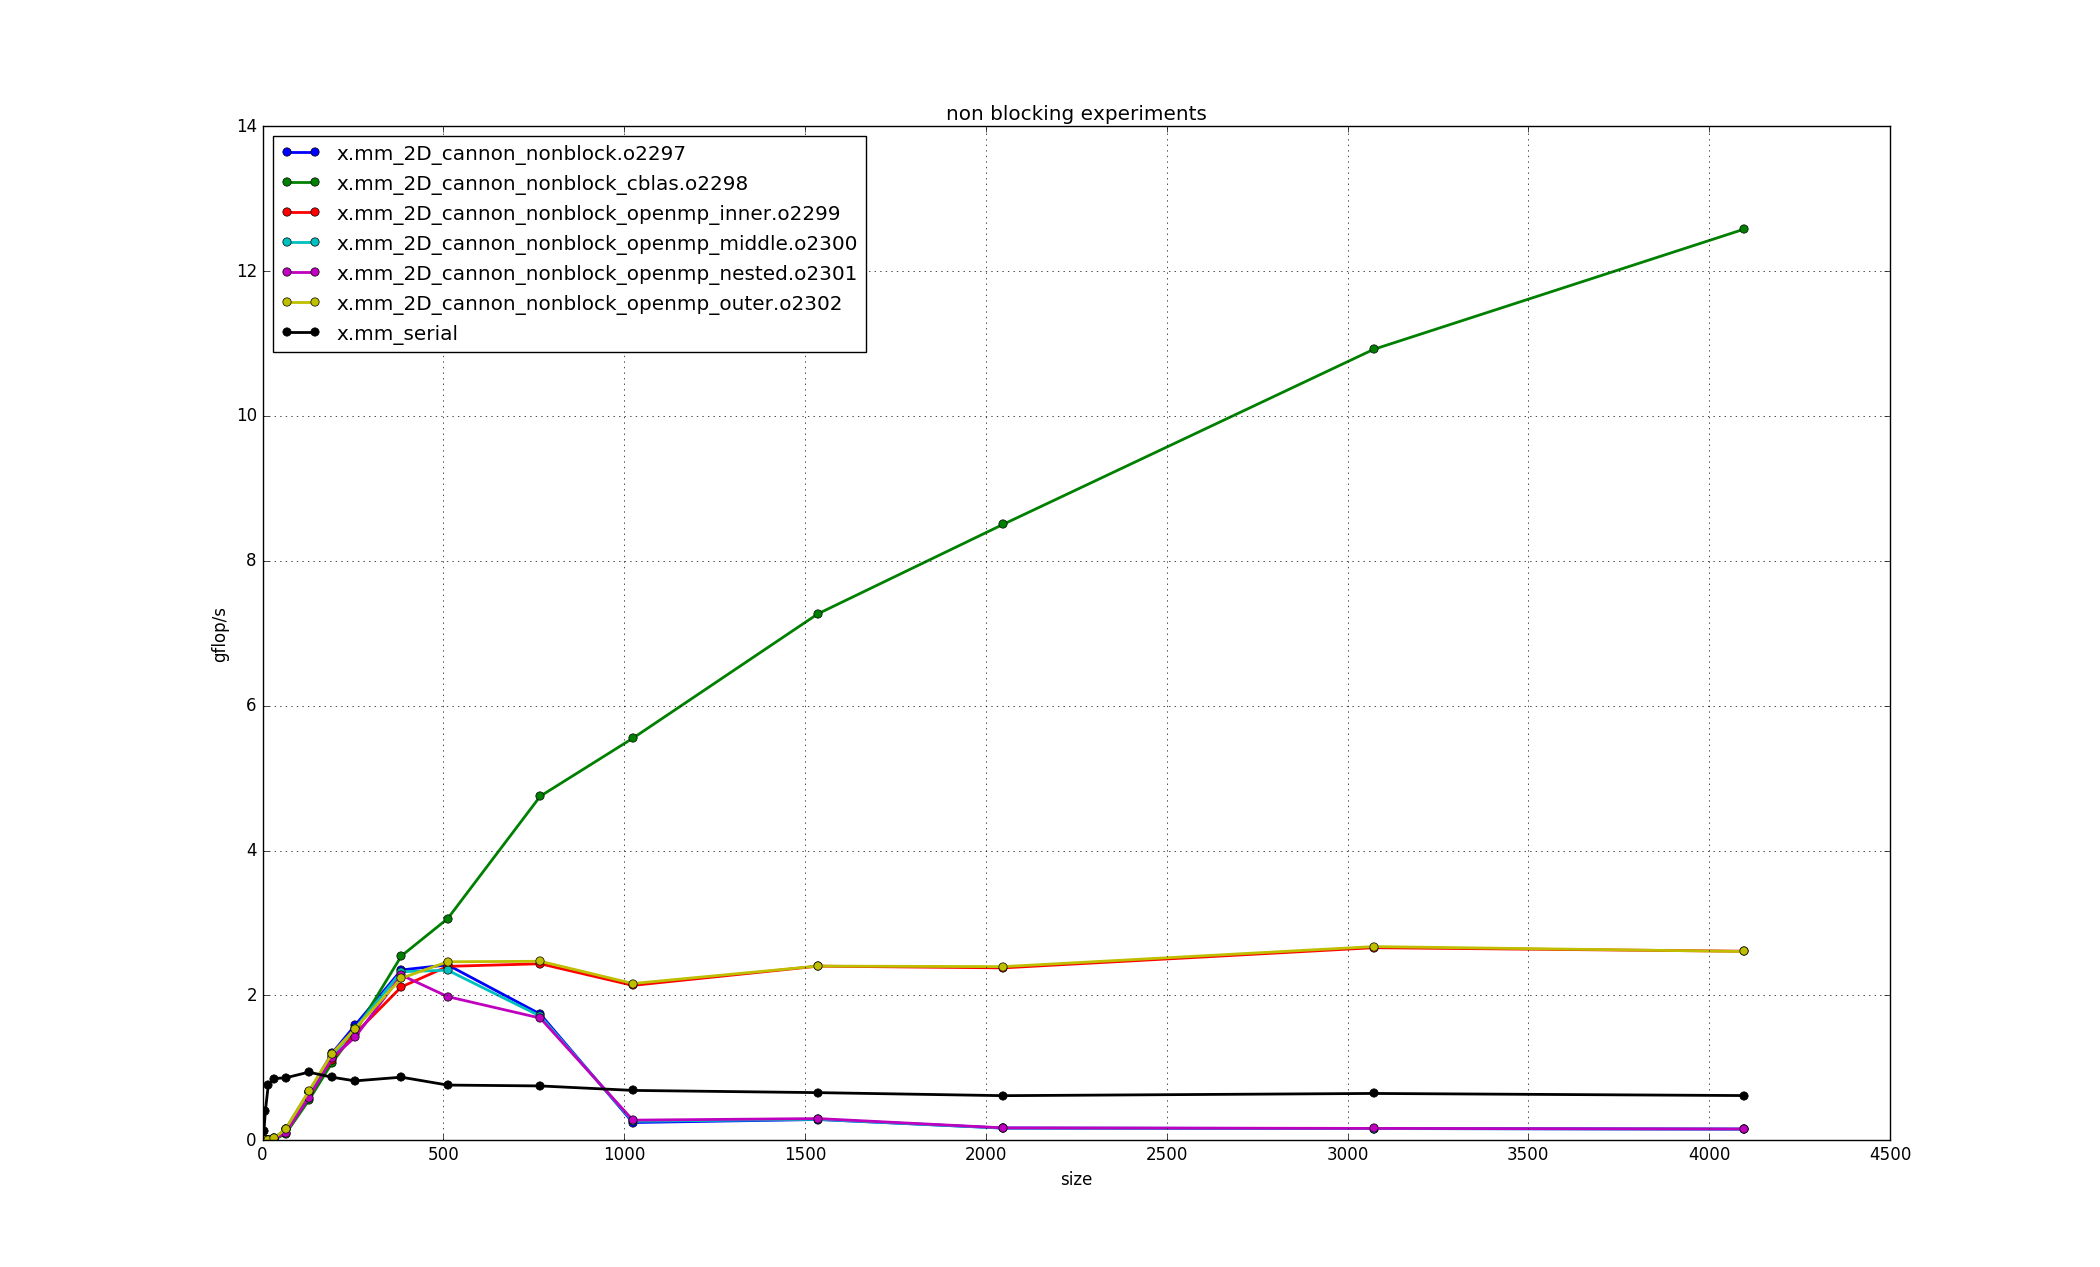
\includegraphics[width=15cm]{immagini/non_blocking_gflops.png}
    \end{center}
    \caption{MM MPI bloccanti: Gflop/s}
    \label{fig:non_blocking_gflops}
\end{figure}

Quello che \`{e} interessante vedere in questi grafici \`{e} l'impatto che le varie ottimizzazioni hanno sull'algoritmo parallelo. In generale una comunicazione non bloccante favorisce le performance e throughput dell'algoritmo e pi\`{u} \`{e} ottimizzata la moltiplicazione locale nel nodo meglio l'algoritmo performa.
